\documentclass[a4paper,12pt]{book}

\usepackage{amsmath}
\usepackage[top=1.0in,bottom=1.0in,left=1.5in,right=1.5in]{geometry}
\usepackage{epstopdf}
\usepackage{hyperref}

\usepackage{amssymb}
\usepackage{graphicx}
\usepackage{braket}
\usepackage{paralist}
\usepackage{eufrak}
\usepackage{amscd}

%% Page Style
\usepackage{fancyhdr}
\pagestyle{fancy}
\renewcommand{\chaptermark}[1]{\markboth{\chaptername\ \thechapter.\ #1}{}}
\renewcommand{\sectionmark}[1]{\markright{\thesection.\ #1}}

\newcommand{\helv}{\fontfamily{phv}\fontseries{b}\fontsize{12}{12}\selectfont}

\fancyhf{}
\fancyhead[LE]{\helv \nouppercase{\rightmark}}
\fancyhead[LO]{\helv \nouppercase{\leftmark}}
\fancyfoot[RO,RE]{\thepage}
\renewcommand{\headrulewidth}{0pt}
\renewcommand{\footrulewidth}{0pt}
\fancypagestyle{plain} {
\fancyhead{} % get rid of headers
}

\usepackage{indentfirst}
\linespread{2.0}

\title{Notes}
\author{Zhu Yong Ting}
\def\bE{{\mathbb{E}}}
\def\bR{{\mathbb{R}}}

\def\eqlaw{{\stackrel{\text{(law)}}{=}}}
\def\tS{{\widetilde{S}}}
\def\tB{{\widetilde{B}}}
\def\tmu{{\widetilde{\mu}}}
\def\tsigma{{\widetilde{\sigma}}}
\def\abs#1{{\left|#1\right|}}
\def\E{{\mathrm{E}\,}}
\def\EE#1{{{\mathrm{E}}\left(#1\right)}}


\def\tX{{\widetilde{X}}}
\def\tM{{\widetilde{M}}}
\def\tx{{\widetilde{x}}}
\def\tm{{\widetilde{m}}}


\allowdisplaybreaks[1]
 
\usepackage{hyperref}

\usepackage{natbib}


\begin{document}
 \bibliographystyle{cje}

\pagestyle{empty}
\maketitle

\pagestyle{fancy}
\pagenumbering{roman}
\tableofcontents 
\listoftables 
\listoffigures
\indent


\chapter{Introduction}
\pagenumbering{arabic}


An {\it option} is a contract which gives the holder the right but not the obligation to buy or sell an underlying asset at or before a certain date at an agreed price, as mentioned in \citeauthor{Hull2008}.
To get this right, the buyer should pay the seller. The price set in the contract is known as the {\it strike price}; the date is known as {\it expiration date} or {\it maturity}. There are always two sides involved in every option contract. On one side is the investor who has bought the option. This side is known as the long position. Another side is the short position who has sold the option. A {\it call} option gives the holder the right to buy the underlying asset, while a {\it put} option gives the holder the right to sell the underlying asset. European options can be exercised only at the expiration date. American options on the other hand may be exercised at any time before the expiration date.

To help the understanding of option, here we can give an example of the use of an option. Suppose that it is now January 15. A copper fabricator expects it will need 100,000 pounds of copper on May 15 to meet a certain contract. The spot price of copper is 140 cents per pound. To fix the expense of raw material, the fabricator may take a long position of a call option, for example, a call option with a strike price of \$120,000 for 100,000 pounds of copper expired in four month. Holding this option, the fabricator eliminates its risk exposure to the changes of copper price. This example is using an option as a hedging instrument. There are other purposes of using of options.

Generally, there are three broad categories of traders of options: {\it hedgers}, {\it speculators}, and {\it arbitrageurs}. Hedgers use options to reduce the risk that they face from potential future movements in a market variable. Speculators use options to bet on the future direction of an asset. Taking advantage of a discrepancy between prices in two different markets, arbitrageurs lock in risk free profits by concurrently taking offsetting positions in two or more markets. Options market have been extraordinary successful. One main reason is that they meet the needs of different types of traders.

Options have a long history. There is evidence that Romans and Phoenicians used similar contracts in shipping.  It is also convinced that Thales, a mathematician and philosopher in ancient Greece, used options to secure a low price for olive presses in advance of the harvest. In the 17th century the Dutch bought and sold options structured on tulip. However, the trading of option actually took off in the later 1970s. The Chicago Board of Trade established the Chicago Board Options Exchange (CBOE) and began trading listed call options on 16 stocks on April 26, 1973.
From this moment on, innovation has bred the creation of copious products tailored to fill the needs of different types of investors. Path-Dependent options, such as Asian options, barrier options and lookback options are traded in market routinely.
Recently, even more exotic types of option such as Parisian option and ${\alpha}$-quantile option have appeared and have attracted interest. Although exotic options are a relatively small part of financial market in terms of volume, these options are important to investment banks because they are generally much more profitable than plain vanilla option.

Options are bought and sold in two ways. Options with standardized terms are traded on organized exchanges. This kinds of options are more standard and liquid than over-the-counter options. Over-the-counter options are not listed in exchanges and instead only quoted by financial institutions. According to the statistics published by Bank for International Settlements, the central bankers' central bank, in June 2009, the amounts outstanding of options traded in organized exchange were 43.75 trillion and the figure for over-the-counter options is 68.19 trillion.

The prosperousness of option market calls for valuation methods of options. While in return, the success of pricing model also boosts the development of options. In chapter 2, we review the fundamental pricing principal for European and American options. The popular numerical methods are surveyed in this chapter 3. In chapter 4, we give an extensive study of $\alpha$-quantile and $\alpha$-quantile option. This is the main focus of our research.

\chapter{Principles of option pricing}

% add more Brodie option pricing: valuation models and applications and the
Usually, there are five factors affecting the price of a stock option:
\begin{enumerate}[1.]
\item The current stock price, $S_0$
\item The strike price, $K$
\item The time to maturity, $T$
\item The volatility of the stock price, $\sigma$
\item The risk free interest rate, $r$
\end{enumerate}

Because exercise is a right but not an obligation, the payoff of an option is always non-negative. For European option, the exercise payoff from a long position is $(S_T - K)^+ = \max \{S_T-K,0\}$. As for American option, the payoff function is similar, what is different is that we should use the stock price when the option is executed to calculate payoff, instead of $S_T$ in European case. 

Usually there are closed form price formulas for European options. In addition numerical approaches can solve this problem, such as binomial tree and Monte Carlo simulation. We will give a brief introduction about these numerical methods later. Because we do not know when American option will be excised, the pricing of American option is more complicated. A complete solution to American option pricing problem should address two aspects, option value and an optimal exercise strategy. Only in a few cases are analytic solutions available. In most cases, numerical approach is needed. For example, \cite{Lim2004} propose an approach to compute both the price and the optimal exercise boundary for American style lookback options.

In this chapter, we give a detailed review about the two major option pricing principles, no arbitrage valuation and risk neutral valuation. The valuation of American options is discussed. Interested reader can find more exhaustive reviews about option valuation models and applications in \cite{2004Broadie}. In addition, because of the similarity between lookback option and $\alpha$-quantile option, the pricing of lookback option is summarized. 

\section{European Options}
\subsection{No-Arbitrage Valuation}

The no-arbitrage principle is the fundamental of pricing of options. \citet*{Black:1973} is the landmark paper in this field. \citet*{merton1973} was the first to expand the mathematical understanding of this options pricing model and used the term "Black-Scholes" options pricing model.

\subsubsection{Black-Scholes framework}
The most popular model to describe stock price behavior is known as Black-Scholes model.
Let $S_t$ be the stock price. Then under this model, $S_t$ satisfies this equation:
\begin{equation}\label{eq:1}
dS_t = \mu S_tdt + \sigma S_tdB_t,
\end{equation}
with $\mu$ and $\sigma $ constant, which represent the expected return on the stock and the volatility respectively. The process $\{B_t\}$ is a standard Brownian motion which represents the underlying uncertainty of the market. There are many other assumptions in this model as following:

\begin{enumerate}[1.]
\item It is possible to borrow and lend cash at a known constant risk-free interest rate.
\item There is no transaction or tax costs.
\item The stock does not pay a dividend.
\item All securities are perfectly divisible. In other words, it is possible to buy any fraction of a share.
\item There are no restrictions on short selling.
\item There is no arbitrage opportunity.
\item Security is trading continuously. This means you can sell or buy security at any time.
\end{enumerate}

These assumptions are usually referred as Black-Scholes framework. Further studies show that many conditions can be relaxed. For simplicity, we follow the Black-Scholes framework in this section.

% This approach to model stock price was first introduced by Black, Scholes and Merton.
% Denote $r$ as the constant continuously compounded risk-free interest rate. Under risk-neutral assumption, we can get $\mu = r $.

\subsubsection{Black-Scholes PDE}
Let $V(S, t)$ be the value of an option at time $t$. The value at maturity $T$, $V(S,T)$ is the payoff. To get its value at an earlier time, we should know how it changes as a function of $S$ and $t$. Suppose $V(S,t)$ is twice differential, applying It$\breve{o}$'s lemma to $V$ we get:
\begin{equation}\label{ito}
dV_t = ( \frac{\partial V}{\partial t} + \frac{\partial V}{\partial S} S_t \mu + \frac{1}{2}\frac{{\partial}^2}{\partial S^2} {S^2}_t {\sigma}^2 ) dt + \frac{\partial V}{\partial S} S_t \sigma d B_t
\end{equation}

As we know, option is based on stock. That is $V_t$ and $S_t$ share the same underlying which means the source of uncertainty is the same for both. Then we can eliminate Brownian motion $B_t$ by constructing certain portfolio of stock $S$ and option $V$. The appropriate trading strategy is holding one option and $ -\frac{\partial V}{\partial S}$ shares of stock.

At time $t$, the value of this portfolio is
\begin{equation}
\Pi = V - \frac{\partial V}{\partial S} S
\end{equation}

The instantaneous profit or loss  $dR$ over time interval $[t, t+dt]$ is
\begin{equation}
dR = dV - \frac{\partial V}{\partial S} dS
\end{equation}

Substituting equation (\ref{ito}) in above we get
\begin{equation}
dR= (\frac{\partial V}{\partial t} + \frac{1}{2}\frac{{\partial}^2 V }{\partial S^2} {S^2}_t {\sigma}^2 ) dt
\end{equation}

This equation does not contain $dB_t$ part, which means that the return of the portfolio is entirely riskless. Black and Scholes interpret this equation as under their ideal conditions, the rate of return on this portfolio must be equal at all times to the rate of return on any other riskless instrument; otherwise, there would exist opportunities for arbitrage. Assuming the risk free rate of return is $r$,  over the time period [t, t + dt] now we have
\begin{equation}
r \Pi dt = dR =  (\frac{\partial V}{\partial t} + \frac{1}{2}\frac{{\partial}^2}{\partial S^2} {S^2}_t {\sigma}^2 ) dt
\end{equation}

From this, we then get the Black Scholes PDE
\begin{equation}\label{black-pde}
\frac{\partial V}{\partial t} + \frac{\partial V }{\partial S} S_t r + \frac{1}{2} \frac{{\partial}^2 V}{\partial S^2} {S^2}_t {\sigma}^2 -rV=0
\end{equation}
Let $f(s)$ be the payoff function of an option, then the boundary conditions for this option is
\begin{equation}\label{Black-boundary}
\begin{cases}
V(S_T,T) =f(S_T)  & \text{on } \bR_+ \\
V(0,t)=f(0)e^{-r(T-t)} & \text{on } [0,T) \\
\displaystyle\lim_{S \to \infty} V(S,t)= f(\infty)e^{-t(T-t)} & \text{on } [0,T)
\end{cases}
\end{equation}

Partial differential equation (\ref{black-pde}) is the fundamental valuation equation for options' price. This PDE applies to all options, regardless its payoff function. For different options, what should change is equation (\ref{Black-boundary}), i.e., boundary conditions.

As suggested, under transformation
\begin{equation}
\begin{cases}
S=K\exp{x} \\
t=T-\frac{\tau}{\frac{1}{2}\sigma ^2} \\
V(S,t)=e^{-\alpha x - \beta \tau } \mu(x, \tau)\\
\alpha=(r-\frac{1}{2} \sigma ^2) / \sigma ^2 \\
\beta= \alpha ^2 + 2r/{\sigma}^2
\end{cases}
\end{equation}
$\mu(x,\tau)$ satisfies the heat equation
\begin{equation}
\frac{\partial \mu}{\partial \tau} = \frac{\partial ^2 \mu}{\partial x^2}
\end{equation}
with the boundary conditions
\begin{equation}
\begin{cases}
e^{-\alpha x} \mu (x,0) = f(K \exp(x)) & \text{on } \bR \\
\displaystyle \lim_{x \to -\infty}e^{-\alpha x- \beta \tau } \mu(x,\tau) = f(0)e^{-2r\tau / \sigma ^2} &\text{on } \tau \in [0,\frac{1}{2}\sigma ^2 T] \\
\displaystyle \lim_{x \to \infty} e^{-\alpha x -\beta \tau } \mu{x,\tau}  = f(\infty) e^{-2r\tau / \sigma ^2} & \text{on } \tau \in [0, \frac{1}{2} \sigma ^2 T]
\end{cases}
\end{equation}

Heat equation was originally used to describe the distribution of heat in a given medium over time, which has been well studied in Physics. If $\lim_{x\to \pm \infty} \mu (x, \tau)= 0$ , the Gaussian density function $\mu (x,t) = (2 \sqrt{\pi t} )^{-1} \exp(-x^2 /{4t})$ with mean $0$ and standard deviation $\sqrt {2t} $ is the fundamental solution.

\subsubsection{Black Scholes Formula}
For European call option, the payoff is $f(S)=(S-K)^+$. Then the valuation formula obtained by Black Scholes PDE is
\begin{equation}
c(S_t,t;K)=S_t N(d(S_t;K,T-t))-Ke^{-r(T-t)}N(d(S_t;K,T-t)-\sigma\sqrt{T-t}),
\end{equation}
where $N(.)$ is the cumulative distribution function of standard normal and
\begin{equation}
d(S_t;K,T-t)=\frac{1}{\sigma \sqrt{T-t}} [\log(\frac{S_t}{K}) + (r+\frac{1}{2}\sigma ^2)(T-t)].
\end{equation}
This formula is known as Black Scholes formula for European call option with strike $K$ and maturity date $T$.

Similarly , the pricing formula for European put option is
\begin{equation}
p(S_t, t;K)= Ke^{-r(T-t)}N(-d(S_t ; K,T-t) +\sigma \sqrt{T-t})-S_t N(-d(S_t;K,T-t)).
\end{equation}

Compare pricing formulas for put and call, we find that they satisfy this equation
\begin{equation}
c(S_t,t;K) + K e^{-r(T-t)} = p(S_t,t;K) + S_t.
\end{equation}
The above relationship between European put and call is called put-call parity. We can get put-call parity by constructing two portfolios. One contains an European call option and $Ke^{-rT}$ cash. Another contains one European put option and one share of the underlying stock. At maturity of the options, both portfolios worth 
\begin{equation}
\max(S_T,K).
\end{equation}
Since European option cannot be exercised before maturity, the two portfolios must have the same value at the beginning. This is the reason why put-call parity holds. Thanks to put-call parity, if we know the price of an European call option, we can deduce the price of put with the same strike price and maturity date, and vice versa.


Further study suggests that some conditions about Black Scholes Model can be extended. Models with transaction fees, short sale constrains and other extensions are available.
%
%% If we define $G = \ln S$, after some calculation, we get
%\begin{equation}\label{eq:2}
%dG_t = \frac{\mu - \sigma ^2 }{2} dt + \sigma dB_t.
%\end{equation}
%%From this we can see that the natural logarithm of stock price is Brownian motion with drift $\mu$, and variance $\sigma^2$. This model implies that the stock's price at a given time $T$ follows lognormal distribution. The standard deviation of the logarithm of the stock price is $\sigma \sqrt{T}$.
%%
%%Black et. al. \cite{Black:1973} pointed out that the proper price of an option should be the expected present value of its payoff. Based on this idea, there are many studies about the pricing of options. For European plain vanilla option, its price can be priced in closed form. As for American plain vanilla option, because it can be executed at any time before maturity, the pricing is much more complicated. In this case, it is an optimal stopping problem. Comparing to vanilla option, there are another school of options called exotic options. Exotic options are nonstandard options created by financial engineers, which usually only traded in over-the-counter market.
%%%In this case, one can deduce that the optimal stopping time is given by some region. Precisely, the holder excises the option when stock price enter some region.



\subsection{Risk-Neutral Valuation}
As revealed in Black-Scholes partial differential equation and corresponding boundary conditions, interest rate $r$, volatility $\sigma$, strike price $K$, stock price $S_0$ and time to maturity, $T$  are all the market parameters that relevant to the price of options. The expected return rate, very surprisingly, does not have any influence on option's price. The Black-Scholes PDE also does not involve any parameter regarding the risk preference of investors. This phenomenon brings hint to another approach of option valuation, risk neutral valuation. 

Risk neutral valuation, first introduced by \citet*{cox-ross1976}, is a very important pricing tool. As a powerful and frequently used pricing theory, risk neutral valuation has been a source of confusion. But the underlying principle can be easily expressed in the binomial case. 

Assume a risky asset whose price is currently $S$ and its price at next period is either $Su$ with probability $q$ or $Sd$ with probability $1-q$. Factors $u$ and $d$ indicate one plus the percentage change in asset price. The real world we live in are risk averse, which is we require extra reward for taking risk. Under this guideline, in risk averse world, any risky asset is priced as discounted value of its future expectation. In our example, the expected future price of this asset is $qSu+(1-q)Sd$. Therefore, the current price of this asset should be 
\begin{equation}
S=\frac{qSu+(1-q)Sd}{1+k}
\end{equation}
where $k$ is the risky discount factor, sometimes known as the required return rate, which usually consists of risk free rate $r$ plus a risk premium. Resorting to the famous capital asset pricing model (CAPM), we can get the risky discount factor. Thus we can get the price of the asset under risk averse world. 

However, with the knowledge of $S$, $u$ and $d$, can we get the price of the asset in a different order ? That is, can we find a new pair probability $p$ and $1-p$ that can substitute $q$ and $1-q$ in the calculation of asset price which allows us to use the risk free interest rate $r$ instead of risky discount factor $k$ ? If  $d < 1+r < u$, that is, in no arbitrage world, the answer is positive. 

When $d < 1+r <u$, if $p$ satisfies $pu+(1-p)d= 1+r$, or equivalently $p=(1+r-d)/(u-d)$, we can write the stock price in following manner: 
\begin{equation}
S=\frac{pSu+(1-p)Sd}{1+r}
\end{equation}

This can be easily proved. Just divide both sides of the above equation by $S$ and multiply with $1+r$. We can get $1+r = pu +(1-p)d$, or its equivalent statement $p=(1+r-d)/(u-d)$. This expression shows that we can 
restate the price of stock by adjusting the probability and discounting it at the risk free rate and what is more,     the only information we need to know in this process is only the volatility and risk free rate. We need make no assumption about investors' attitude towards risk. This method works on risk aversion, risk neutral and risk seeking investors, regardless their risk preference. A world where all individuals are indifferent to risk is called {\it risk neutral world}. In this world investors do not demand compensation for taking risk and the expected return for any financial product in risk neutral world is the risk free rate.

Above is the basic idea of a important derivative pricing principle called {\it risk neutral valuation}. The probability $p$ used to calculate expectation in risk neutral world is known as {\it equivalent martingale probability}. With the help of more advanced mathematics, risk neutral valuation remains valid and useful in the situation with stochastic interest rate and volatility. Interesting study about this model can be found in \cite{HarrisonKreps1979}, \cite{Harrison1981} and \cite{Kreps1981}.

\section{American Options}
In the risk neutral world, the price of American options has an easy 
expression. At time $t$, the price of American Option is
\[
V_t(S_t) =\sup_{t\leq \tau\leq  T}Ee^{-r(\tau-t)}f(S_\tau),
\]
where $\tau$ are any stopping time stops before $T$ and
\[
f(s,t) = 
\begin{cases}
(s-K)^+ & \text{for call option}\\
(K-s)^+ & \text{for put option}
\end{cases}
\]
is the payoff function as usual.
This is an optimal stopping problem. 

We can understand this formula by noticing that $\tau$ corresponds to possible strategy to execute the option. More precisely, the holder will execute the option at time $\tau$. The price is given by the optimal strategy. 

It can be proved that the optimal strategy is given by some region $D$ in $(S,t)$ plane, i.e. $\tau<t$ if and only if $(S_t,t)\in D$. This domain $D$ is called as execute region. 

It has a systematic way to translate this optimal stopping problem into PDE. However it is also interesting to derive the PDE directly, just as the way we derive the Black-Scholes equation.

Let $V(S,t)$ be the price of an American option. Let us consider call option. Before execute the option, $C(S,t)$ should satisfy the usual Black-Scholes equation. When, the stock price is high, especially, $(S-K)^+\geq V(S,t)$, the holder should execute the option, otherwise there will be an arbitrage opportunity. We get a free boundary problem:
\[
\begin{cases}
\frac{\partial V}{\partial t} + \frac{\partial V }{\partial S} S_t r + \frac{1}{2} \frac{{\partial}^2 V}{\partial S^2} {S^2}_t {\sigma}^2 -rV=0\\
V(S, T) = f(S)\\
\frac{\partial V}{\partial S}(S,t) = +1 \text{ at the boundary} 
\end{cases}
\]

In fact $\frac{\partial V}{\partial S}(S,t) = +1$ is a smoothness condition, since we have $\frac{\partial}{\partial S}(S-K)^+ = 1$ when $S$ big enough.  

\section{Lookback options}
Lookback option is a type of exotic options whose prices have path dependency effects. 
Lookback options give the hold the right to capture the difference between asset price when the option is executed and maximum or minimum asset price reached during the life of the option.  According to the difference in the selection of strike price, you can find two styles of Lookback options : floating strike lookback and fixed strike lookback.

\subsection{Floating strike lookback option}
As you can see from the name, the strike price of this kind lookback is floating and is determined at the end of the option's life, which is at maturity. For a European style lookback call option with floating strike, the payoff is the amount that the final asset price exceeds the minimum asset price attained during the life of the option. The payoff function is 
\begin{equation}
LC_{floating} = S_T - S_{\min}
\end{equation}
where $S_{\min}$ is the minimum asset's price occurred during the life of the option.

As for the put option, the payoff is the amount by which the maximum asset price attained during the life of the option exceeds the final asset price. Payoff function for floating put is given as
\begin{equation}
LP_{floating}=S_{\max}-S_T
\end{equation}
where $S_{\max}$ is the maximum asset's price during the life of the option. 

A lookback floating call option gives the holder the right to buy the underlying at the lowest price during the life of a option. While the put provides the holder one way to sell at the highest price during the life of a option. 

One interesting fact of floating lookback is that this kind option is never out of the money. Therefore holders of this type option will always excise it at maturity. This fact, it is always in the money, makes it more expensive than plain vanilla options. 

\cite{Goldman1979} firstly provided the valuation formulas for European floating lookbacks. In \cite{Hull2008}, the value of a this type call option is
\begin{equation}\label{eq:3}
S_0e^{-qt}N(a_1) - S_0 e^{-qT}\frac{\sigma ^2}{2(r-q)} N(-a_1) - S_{\min} e^{-rT}(N(a_2) - \frac{\sigma^2}{2(r-q)} e ^{Y_1} N(-a_3)
\end{equation}
where
\begin{equation}\label{eq:4}
\begin{split}
a_1 &=\frac{\ln(S_0 / S_{\min}) + (r-q+\sigma^2 /2)T}{\sigma \sqrt{T}}\\
a_2 &= a_1 - \sigma \sqrt{T}\\
a_3 &= \frac{ln(S_0 / S_{\min})+ (-r+q+\sigma^2 / 2)T}{\sigma \sqrt{T}}\\
Y_1 &= - \frac{2(r-q-\sigma^2 / 2) \ln(S_0 / S_{min})}{\sigma^2}
\end{split}
\end{equation}
and $S_{\min}$ is the minimum asset price achieved to date.
The value of a European lookback put is
\begin{equation}\label{eq:5}
S_{\max} e^{-rT} ( N(b_1) - \frac{\sigma^2}{2(r-q)} e^{Y_2} N(-b_3)) + S_0 e^{-qT}\frac{\sigma^2}{2(r-q)} N(-b_2) - S_0 e^{-qT} N(b_2)
\end{equation}
where
\begin{equation}\label{eq:6}
\begin{split}
b_1 &= \frac{\ln(S_{\max} / S_0) + (-r + q + \sigma^2 /2)T}{\sigma \sqrt{T}}\\
b_2 &= b_1 - \sigma \sqrt{T}\\
b_3 &= \frac{\ln(S_{\max} / S_0) + (r-q-\sigma^2 /2)T}{\sigma \sqrt{T}}\\
Y_2 &= \frac{2(r-q-\sigma^2 / 2) \ln(S_{\max} / S_0)}{\sigma^2}
\end{split}
\end{equation}
and $S_{\max}$ is the maximum asset price achieved to date.



The formulas above are got under the assumption that the asset price is observed continuously. However, in real life, the asset price is observed discretely. \cite{Broadie1999} give a correction to these formulas to deal with discrete situation.

For the discrete options, let $m$ be the number of price-fixing dates and $\Delta t= T/m$ the interval between fixing. In their paper, we can find that the price of a discrete lookback at the $k-th$ fixing date and the price of a continuous lookback at time $t = k \Delta t$ satisfies
\begin{equation}\label{eq:7}
V_m (S_\pm)
=
\pm[e^{\mp\beta_1 \sigma \sqrt{\frac{T}{m}}}
V(S_{\pm}e^{\mp\beta _1 \sigma \sqrt{\frac{T}{m}}}) +
(e^{\mp \beta_1 \sigma \sqrt{\frac{T}{m}}} -1)S_t ]+ o(1/\sqrt{m})
\end{equation}
where, in $\pm$ and $\mp$, the top case applies for puts and the bottom for calls, and $\beta_1 = \lim_{m\to\infty} \frac{\sqrt{m}E[\max_{0\leq t \leq T} B_t - \max_{0\leq k \leq m} B_{kT/m}]}{\sigma \sqrt{T}}$.

By this correction, we can use continuous pricing formula
to value discrete lookback. To get a more precise value for put,
first we should inflate the predetermined max by a factor of
$e^{\beta_1 \sigma \sqrt{T/m}}$,
then deflate the expected maximum over $[0,T]$ by the same factor. For a lookback call, first deflate the predetermined minimum, then inflate the expected minimum.

\subsection{Fixed strike lookback option}
Similar to plain vanilla options, lookback option's strike price also can be fixed. The difference, comparing with standard European option, is that fixed lookback is not exercised at the price at maturity.  Instead, the payoff is the optimal difference between the underlying asset price and strike price. 

For a fixed lookback call option, the holder is allowed to calculate the payoff using the highest underlying asset price obtained before maturity. As for fixed lookback put option, the holder can use underlying asset's lowest price. One can find that the intrinsic value of fixed strike lookback in never decreasing as time passes. The payoff functions for fixed Lookback call and  Lookback put respectively are:
\begin{equation}
LC_{fixed} = \max\{S_{\max} - K, 0\} 
\end{equation}
\begin{equation}
LP_{fixed}= \max\{K-S_{\min},0\}
\end{equation}
where $K$ is the strike price.

The pricing formula of fixed strike lookback is given by \cite{Conze1991} using risk neutral pricing valuation method. Under risk neutral pricing frame, the value of a call is 
\begin{equation}
LC_{fixed} = e^{-rT}E[(S_{\max}-K)^{+}].
\end{equation}
This leads to 
\begin{equation}
\begin{split}
LC_{fixed} =& S_0 N(d) - e^{-rT}KN(d-\sigma \sqrt{T}) \\
&+ e^{-rT} \frac{\sigma^2}{2r} S_0 [ -{(\frac{S_0}{K})}^{-\frac{2r}{\sigma^2}} N(d-\frac{2r}{\sigma}\sqrt{T}) + e^{rT}N(d)].
\end{split}
\end{equation}
In the case that $K\geq S_0$, or otherwise
\begin{equation}
\begin{split}
LC_{fixed} = & e^{-rT}(S_0 - K) + S_0 N(d') - e^{-rT}S_0 N(d'-\sigma \sqrt{T}) \\
&+ e^{-rT} \frac{\sigma ^2}{2r} S_0 [ -N(d'-\frac{2r}{\sigma}\sqrt{T}) + e^{rT}N(d')]
\end{split}
\end{equation}
where
\begin{equation}
d = (ln\frac{S_0}{K} + rT + \frac{1}{2} \sigma^2 T)/ {\sigma \sqrt{T}}
\end{equation}
and
\begin{equation}
d'=(rT + \frac{1}{2} \sigma^2 T)/ {\sigma \sqrt{T}}.
\end{equation}

Similarly, the value of the put is 
\begin{equation}
\begin{split}
LP_{fixed} =& -S_0 N(-d) + e^{-rT} KN(-d + \sigma \sqrt{T})  \\
&+ e^{-rT} \frac{\sigma^2}{2r} S_0 [ (\frac{S_0}{K})^{-\frac{2r}{\sigma^2}}N(-d+\frac{2r}{\sigma}) - e^{rT}N(-d)]
\end{split}
\end{equation}
if $K\leq S_0$, otherwise
\begin{equation}
\begin{split}
LP_{fixed} = & e^{-rT} (K-S_0) - S_0 N(-d') + e^{-rT}S_0 N (-d' + \sigma \sqrt{T}) \\
&+ e{-rT} \frac{\sigma^2}{2r} S_0 [ N(-d' + \frac{2r}{\sigma} \sqrt{T}) -e^{rT}N(-d')]
\end{split}
\end{equation}
 
\subsection{American lookback option}

As for American option, the complete solution should provide both the option value and an optimal exercise strategy. Due to this complicity, usually we need use numerical approach to solve the problem of pricing American style lookback option. In \cite{Lim2004}, for American \emph {fixed strike} lookback option they provide an full approach to compute the price and the optimal exercise boundary. In that paper, they first propose a space-time transformation which can reduce the valuation of a group of American lookback options to a single canonical optimal stopping problem for standard Brownian motion. Under this transformation, calendar time is scaled by square of volatility. Therefore, the canonical time horizon is only a small part of time to expiration. In addition, the transformation also removes the dependence on a prescribed root node which then makes computing the entire early excise boundary by backward induction possible.

%Fix a process $X_t$, define $M_t = \max_{0\leq s\leq t} X_s$.
%When $X_t$ is a standard brownian motion without drift,
%the joint distribution of $M_t$ and $X_t$ can be easly calculated by reflection principle\cite{Karatzas91}:
%\[
%P(X_t \in a+dx, M_t \in b+dm) =
%\]

\chapter{Numerical Methods}

For American, and path-dependent options, generally closed form pricing formulaes are not available. In this case,usually numerical methods may be required. Even for Black Scholes formula, in practice, integration and the normal probability are obtained numerically. In this chapter, we provide a brief summary of the major numerical methods for option pricing. The most popular numerical approaches are lattice method, finite difference and Monte Carlo simulation. Generally speaking, different numerical methods are applicable in different situations. 

\section{Lattice Methods}
Lattice methods, also known as tree methods, use discrete time and discrete state approximations of the evolvements of underlying assets to calculate option prices. The lattice method was originally proposed in \cite{cox1979}. Lattice approaches are popular because lattice methods are easy to understand and implement. In risk neutral valuation framework, as we discussed, the underlying price follows $S_{t+h} = S_t e^{Z}$, and $Z\sim N((r-\frac{1}{2} \sigma ^2)h,\sigma ^2 h)$. In lattice method, over a discrete time interval, one discrete random variable $X$ is used to approximate $Z$. $X$ takes value as $x_i$ with probability $p_i$ $i=1,2,...,m$. If $m=2$, it is binomial tree; If $m=3$, it is trinomial method. The value of the parameters of the distribution of the discrete random variable $X$ are chosen to approximate the distribution of continuous random variable $Z$ exactly or consistently. Under risk neutral method, the value of an option is the discounted present value of the expectation of the option's payoff. In lattice method we first use discrete diagram to approximate the continuous path of the price of underlying asset. Then calculate the discrete expectation of payoff as an approximation of option price. Due to the simplicity of lattice method, adjusted lattice methods for models with dividends, barriers and other complicated features can be easily constructed. However, the key issue of lattice method is the tradeoff between speed and accuracy. 

There are plenty of proposals for tree methods. The popularly used are \cite{cox1979},\cite{jarrow1983},\cite{Boyle1986} and \cite{Amin1991}. 
\begin{table}[htdp]
\caption{Well known Lattice Methods}
\begin{center}
\begin{tabular}{|l|l|l|}
\hline
Lattice & Approximation   & Probabilty \\
\hline
\cite{cox1979} & $x_1= \sigma\sqrt{h}$ & $p_1 =\frac{e^{rh}-e^{-\sigma\sqrt{h}}}{e^{\sigma\sqrt{h}}-e^{-\sigma\sqrt{h}}}$ \\
   &  $x_2=-\sigma\sqrt{h}$& $1-p_1$ \\
\hline
\cite{jarrow1983} & $x_1 = (r-\sigma^2 /2)h+\sigma\sqrt{h}$ & $p_1 = \frac{e^{\sigma^2 h/2}-e^{-\sigma\sqrt{h}}}{e^{\sigma\sqrt{h}}-e^{-\sigma\sqrt{h}}}$ \\   
& $x_2 =(r-\sigma^2 /2)h - \sigma\sqrt{h}$ & $p_2 = 1- p_1$ \\
\hline
\cite{Boyle1986} & $x_1 = \lambda\sigma\sqrt{h}$ & $p_1 = \frac{1}{2\lambda^2} + \frac{(r-\sigma^2 /2)\sqrt{h}}{2\lambda\sigma}$ \\
 & $x_2 = 0$ & $p_2 = 1-\frac{1}{\lambda^2}$ \\
 & $x_3 = -\lambda\sigma\sqrt{h}$ & $p_3 = \frac{1}{2\lambda^2} - \frac{(r-\sigma^2 /2)\sqrt{h}}{2\lambda\sigma}$\\
\hline
\cite{Amin1991} & $x_1 =(r-ln(cosh(\sigma\sqrt{h})))h + \sigma\sqrt{h}$ & $p_1 = 1/2$ \\
& $x_2 = (r-\ln(\cosh(\sigma\sqrt{h})))h-\sigma\sqrt{h}$ & $p_2 = 1/2$ \\
\hline
\end{tabular}
\end{center}
\label{default}
\end{table}%

\section{Monte Carlo Simulation}
As we discussed in Risk Neutral pricing method, option valuation often end to the calculation of an expected value of a certain discounted payoff. For some cases, we can do this computation explicitly. The Black Scholes formula is a example of this class. But for most of the time, we need the help of numerical methods. Monte Carlo simulation is a natural proposal to calculate expectation. Monte Carlo method is very useful to price options with multiple underlying assets. This method is first used to evaluate a European option by \cite{Boyle1977}. 

Generally, Monte Carlo method is done in following steps: 
\begin{enumerate}[1.]
\item 
Generate sample paths for the underlying random variables in question according to the risk neutral measure. 
\item
Calculate the corresponding discounted payoff for each sample path.
\item
Calculate the average discounted payoff on all the samples.
\end{enumerate}

The sharp advantage of Monte Carlo method lies in its convenience in calculation high dimensional integrations. 
The convergence of Monte Carlo is guaranteed by large number theory. Now the focus of the study is on improving the  computational efficiency. Interested readers can find detailed survey on this method in \cite{Boyle1997} and \cite{Glasserman2004}. 



\chapter{$\alpha$-quantile and $\alpha$-quantile option}
For a stochastic process $X_t$,
the $\alpha$-quantile $( 0 \leq \alpha \leq 1)$
is defined by
\[
M(\alpha,t)(\omega) = \inf\Set{x:\int_0^t 1_{(X_s (\omega)\leq x)} > \alpha t}.
\]
Then we can see that $\inf_{0\leq s \leq t}  X_s = lim_{\alpha\to 0}M(\alpha,t)$ and $\sup_{(0\leq s \leq t})  X_s = lim_{\alpha\to 1} M(\alpha, t)$. %In this sense $\alpha$-quantile option can be considered as a general class of lookback option. Unlike lookback option whose payoff depends on the maximum or minimum of the price of stock before maturity as mentioned before, $\alpha$-quantile option's payoff depends on the quantile of the stock price process. This option was first introduced by \cite{Miura} in 1992. \cite{Akahori1995} gave a generalized arc-sine law for this type of options by Feynman-Kac formula.
When $X_{t}$ is a Brownian motion $B_t$, using Feynman-Kac, Dassios obtained the explicit density of $\alpha$-quantile and gave a exceptional representation of the distribution of quantile. In \cite{Dassios1995}, for $\alpha\in[0,1]$, $t\leq 0$, Dassios proved that
\begin{equation}\label{eq:Dassios}
M(\alpha, t) \eqlaw \sup_{s \leq \alpha t} X_s + \inf_{s\leq (1-\alpha)t} X'_s ,
\end{equation}
where $X'$ is a independent copy of $X$. Later \cite{EmRoge1995} gave two proofs of this theorem without using Feynman-Kac computations.

\section{$\alpha$-quantile}
\subsection{The distribution function of $\alpha$-quantile of Brownian motion}
In 1995, Yor gave the distribution function of the $\alpha$-quantile of Brownian motion without drift in \cite{Yor1995}. He obtained this result by simplifying related integral expressions in \cite{Miura}. When $\mu = 0$, that is Brownian motion $B_t$ is without drift, define $\theta = ((1 - \alpha)/(\alpha))^{1/2}$, for the Brownian quantiles on time interval $[0, 1]$,  in \cite{Yor1995} we find:
\begin{equation}
P(M(\alpha,1)\in dx)= \begin{cases}
\sqrt{2 / \pi}exp(-x^2 / 2) \Phi(|x| / \theta)dx  &  \text{if } x \leq 0 \\
\sqrt{2 / \pi}exp(-x^2 / 2) \Phi(\theta x)dx  &  \text{if } x \geq 0
\end{cases}
\end{equation}
where
\begin{equation}\label{eq:density}
\Phi (x) = \sqrt{2/ \pi} \int^{\infty}_x dy exp(-y^2 / 2) = P (|N| \geq x)     (x \geq 0),
\end{equation}
with $N$ a standard Normal random variable.


When $u \neq 0$,  \cite{Dassios1995} addressed this question for a more general case.  As stated in equation (\ref{eq:Dassios}), the distribution of $M(\alpha , t)$ can be represented in terms of the maximum and minimum of process $\{X_t\}$. Therefore we can get the density function of $M(\alpha, t)$ expressed as the convolution of other two density functions.

Denote $g(x; \alpha , t)$ as the density function of $M(\alpha , t)$, in \cite{Dassios1995}, we find that
\begin{equation}\label{eq:fulldensity}
g(x; \alpha , t) = \int^{\infty}_{-\infty} g_1 (x-y; \alpha t) g_2 (y; (1-\alpha) t)dy ,
\end{equation}
where
\begin{equation}
g_1 (x;t) = \begin{cases}
\frac{1}{\sigma}({\frac{2}{\pi t}})^{1/2}exp\{-\frac{(x-\mu t)^2}{2\sigma ^2 t}\} \\
\quad - \frac{2\mu}{\sigma ^2} exp(\frac{2\mu x}{\sigma ^2})[1- \Phi (\frac{x+\mu t}{\sigma \sqrt{t}})], & x \geq 0 \\
0 , & x  < 0 
\end{cases}
\end{equation}

\begin{equation}
g_2 (x;t) = \begin{cases}
0, & x > 0 \\
\frac{1}{\sigma}({\frac{2}{\pi t}})^{1/2}exp\{-\frac{(x-\mu t)^2}{2\sigma ^2 t}\} \\
\quad + \frac{2\mu}{\sigma ^2} exp(\frac{2\mu x}{\sigma ^2}) \Phi (\frac{x+\mu t}{\sigma \sqrt{t}}) , & x \leq 0
\end{cases}
\end{equation}


\subsection{The joint distribution of Brownian motion and $\alpha$-quantile}
In this section we are going to provide the joint distribution of Brownian motion and its quantile. When the Brownian motion is without drift,
ie $\mu = 0 $,
As we know the joint distribution of running maximum and end point of
standard Brownian motion at time $\tau$ is
\[
P(X_\tau\in da, M_\tau\in db) =
\frac{2(2b-a)}{\sqrt{2\pi \tau^3}} \exp(-\frac{(2b-a)^2}{2\tau})
I_{\Set{a\leq b, b\geq 0}} (a,b) da db \triangleq p_\tau(a,b)
\]

To deal with the distribution of $\alpha$-quantile, we use two copy of
Brownian motion and denote corresponding value at
$\tau=\alpha t$(respectively $\tau=(1-\alpha) t$) by $X_1$(respectively $X_2$) and
the corresponding maximum as $M_1$(respectively $M_2$).
Then
\[
\begin{split}
(X_1,M_1, X_2, M_2) \sim& P(X_1\in dx_1, M_1\in dm_1, X_2\in dx_2, M_2\in dm_2)\\
&= P_{\alpha t}(x_1, m_1) P_{(1-\alpha)t}(x_2,m_2) dx_1dm_1dx_2dm_2
\end{split}
\]


Use the transform
\[
\begin{pmatrix}
X_1\\ X_2\\ M_1\\ M_2\\
\end{pmatrix}
\overset{
\begin{pmatrix}
1 & 1 & 0 &0 \\
1 & -1 & 0 & 0 \\
0 & 0 & 1 & 1\\
0 & 0 & 1 & -1\\
\end{pmatrix}
}{\longrightarrow}
\begin{pmatrix}
X_1+X_2\\
X_1 - X_2 \\
M_1 + M_2 \\
M_1 - M_2 \\
\end{pmatrix}
\triangleq
\begin{pmatrix}
X \\ \tX\\ \tM \\M
\end{pmatrix}
\]

And
\[
(X, \tX, M, \tM) \sim \frac{1}{4} P_{\alpha t}(\frac{x+\tx}{2},\frac{m+\tm}{2})
P_{(1-\alpha)t}(\frac{x-\tx}{2},\frac{\tm-m}{2}) I_D,
\]
where $D$ is the domain $\Set{x_1\leq m_1, x_2\leq m_2, m_1 >0, m_2>0}$


Hence 
\[
\begin{split}
&P(M_{\alpha,t}\in dm, X_t \in dx) = P(M_1-M_2\in dm, X_1+X_2\in dx) \\
=& \frac{1}{4} \int_{-\infty}^{\infty}\int_{-\infty}^\infty
P_{\alpha t}(\frac{x+\tx}{2},\frac{m+\tm}{2})
P_{(1-\alpha)t}(\frac{x-\tx}{2},\frac{\tm-m}{2}) I_D d\tx d\tm\\
= & \int_{-\infty}^{\infty}\int_{-\infty}^\infty
P_{\alpha t}(x',m')
P_{(1-\alpha)t}(x-x',m-m') I_{D'} d\tx d\tm\\
= & \int_{\max\Set{0,m}}^{\infty} \int_{x+m-m'}^{m'}
P_{\alpha t}(x', m') P_{(1-\alpha)t}(x-x',m'-m) dx' dm',
\end{split}
\]
where domain $D' = \Set{x' \leq m', x-x'\leq m'-m, m'>0, m'-m>0}$.

\subsection{Euler scheme and random walk}\label{s:euler}
%%Another approach to price quantile option is Monte Carlo simulation. In this method, we need to use the inverse function of the cumulative distribution function of $\alpha$-quantile. When the brownian motion is without drift, 

Sometimes to get the integration of certain stochastic process, we are only able to get the value numerically. For example, if we need to know $\int^T_{0} M(\alpha , t)dt$. Usually we need to simulate a discretized version of the Brownian motion $\{B_t\}$. And the do the calculation based on the simulated sample. Obviously, the accuracy of this approximation is closely related to the length of the discretized time increment, which we denote as $\Delta t= \frac{T}{N}$. Then the questions arise: how fine should the discretization length should be in order to get a satisfied approximation and whether we can quantify the accuracy of this type of simulation. 

The most straightforward approach to get a simulation of $M(\alpha , T)$ is to apply the Euler approximation. In this method, we first get a sample of $\{B_{n \Delta t}\}$, $0\leq n \leq N$. Then we arrange the sample in ascending order and find the $k= \lfloor \alpha  N\rfloor$-th number as an discretized approximation of $M(\alpha , T)$. We denote $M(k, N)$ the approximation of $\alpha$-quantile under Euler scheme. The absolute error 
\begin{equation}\label{strong}
E\|M(\alpha, T)-M(k,N)\|_2
\end{equation}
is one popular measure of the quality of estimation and here $\|\;\| _2$ is the Euclidean distance. If (\ref{strong}) is $O(\Delta t^\gamma)$ as $\Delta t \downarrow 0$, this approximation is claimed to {\it converge strongly} with order $\gamma > 0 $. Strong convergency is important when fine pathwise approximation is need. Meanwhile, an approximation {\it converges} weakly with order $\beta > 0$ if, for any function continuous and $g: \bR \to \bR$ such that all derivatives up to and including $\lceil 2(\beta + 1) \rceil$ exsit and have polynomial growth, 
\begin{equation}
|Eg(M(\alpha,T)) - Eg(M(k, N))| = O (h^\beta) 
\end{equation}
as $h \downarrow 0$. Weak approximation is of importance when only an estimation of the probability distribution of $M(\alpha, T)$ is essential. 

We are interested in the discretization error of Euler scheme for $\alpha$-quantile. Here we present a numerical study of the convergency of Euler scheme. 
%Since usually the knowledge of distribution is already enough to solve many questions, we focus on the weak convergency. 
For our one dimensional problem, the strong convergence measure can be restated as 
\begin{equation}
E|M(\alpha, T)-M(k,N)|
\end{equation}
Because the lack of theoretical study on the discretized quantile, we are not able to give a theoretical conclusion on the strong convergency. Instead, here we present a numerical study of the strong convergency. 

The most challenging part of the design of this experiment is that the samplings of continuous $\alpha$-quantile $M(\alpha, T)$ and the discretized $\alpha$-quantile obtained under Euler scheme $M(k,N)$ should share the same path. The reason is because the discretized error is an expectation. Therefore the traditional method to get samples for continuous random variable, Monte Carlo simulation, is not helpful any more. To address this phenomenon, we use a much finer Euler approximation, in our example $\Delta t = \frac{1}{2^{27}}$, as an approximation of the continuous  $\alpha$-quantile $M(\alpha, T)$. 

The parameter setting is : 
\begin{equation}
\mu = 0 ; \sigma = 1; T=1; N = 2^b , 2^{b+1} , ... 2^{d} ; X_0 = 0; 
\alpha_j =  \frac{1}{2} + \frac{j}{2^b} , j = 0, 1 , 2..., 2^{b-1}
\end{equation}

The algorithm: 
\begin{enumerate}[1.]
\item Generate $2^{d}$ normal random sample $\Set{X_i}$ 
  with mean $\tmu=\mu/2^d$ ,
  $\tsigma = \sigma \sqrt {\frac{T}{2^b}}$  starting with $B_0 = 0$,
  add them up according to time and record them as
  $B_k = \sum_{1\leq i \leq k} X_i$.
\item Calculate the $\alpha_j$ quantiles 
  $M_{j,s}\triangleq M_{\alpha_j 2^s,2^s}$ for sequence 
  $\Set{B_k|k=i 2^{d-s}, 1\leq i\leq 2^{s}}$, where $b\leq s \leq d$. 
\item Use $M_{j,d}$ as the continuous quantiles $M(\alpha_j , T)$.
\item Repeat the above for $L$ times,
  get a sequence of data $\Set{M_{j,s}^{(l)}}_{1\leq l\leq L}$
\item Calculate the mean of errors for $s < d$ using:
\begin{align}
Err^{abs}_{j,s} &= \frac{1}{L}\sum_{1\leq l \leq L} \abs{M_{j,s}^{(l)}- M_{j,d}^{(l)}}
\end{align}
\end{enumerate}

We realize this algorithm for $d=27$,$b=6$ and generate more than 2000 sampled paths. The results are showed in Figure \ref{f:ab}. We are dealing with $\mu = 0$ currently. By the symmetric effect of Brownian motion without drift. We only examine $\alpha$-quantiles where $\alpha$ vary from $[50\%,100\%]$. It is well known that the convergence rate of Euler scheme for Brownian motion is $1$. While the convergence rate of Euler Scheme for the maximum of Brownian motion is $\frac{1}{2}$. Then it seems reasonable to guess that the convergence rate for $\alpha$-quantiles of Brownian motion decrease from $1$ to $\frac{1}{2}$ as the value of $\alpha$ vary from $100\%$ to $50\%$. However, numerical results shows that the convergence rate for $\alpha$-quantile do not work that way. Figure \ref{f:ab} shows that there exists a big difference between the convergence patterns for the maximum of Brownian motion and other $\alpha$-quantiles of Brownian motion. On the other hand, the convergence patterns for different $\alpha$-quantiles are quite similar when $\alpha$ varies from $[50\%, 100\%)$. 

In Figure \ref{f:ab}, the horizontal index $s$ means that the result is obtained on a path in which we divide the whole path on time interval $[0,T]$ into $2^{j}$ equal small intervals. Then to examine the convergence patterns for the increase of denseness on a apple to apple case, we should take logarithm of the errors. The similarity of convergence patterns of $\alpha$-quantiles when $\alpha$ is between $[50\%, 100\%)$ is more obvious after we take the logarithm. 

In Figure \ref{f:lab}, you can see that except for the maximum, i.e. the $100\%$-quantile, the convergence rates of other $\alpha$-quantiles of Brownian motion are close to each other. This is reflected as the lines parallel to each other. Figure \ref{f:ratio} is the convergence rate for different $\alpha$-quantiles. You can see that the convergence rate for $100\%$-quantile is close to $\frac{1}{2}$, while convergence rates for other quantile are centered on $0.75$.  
\begin{figure}[p]\label{f:ab}
   %\centering
   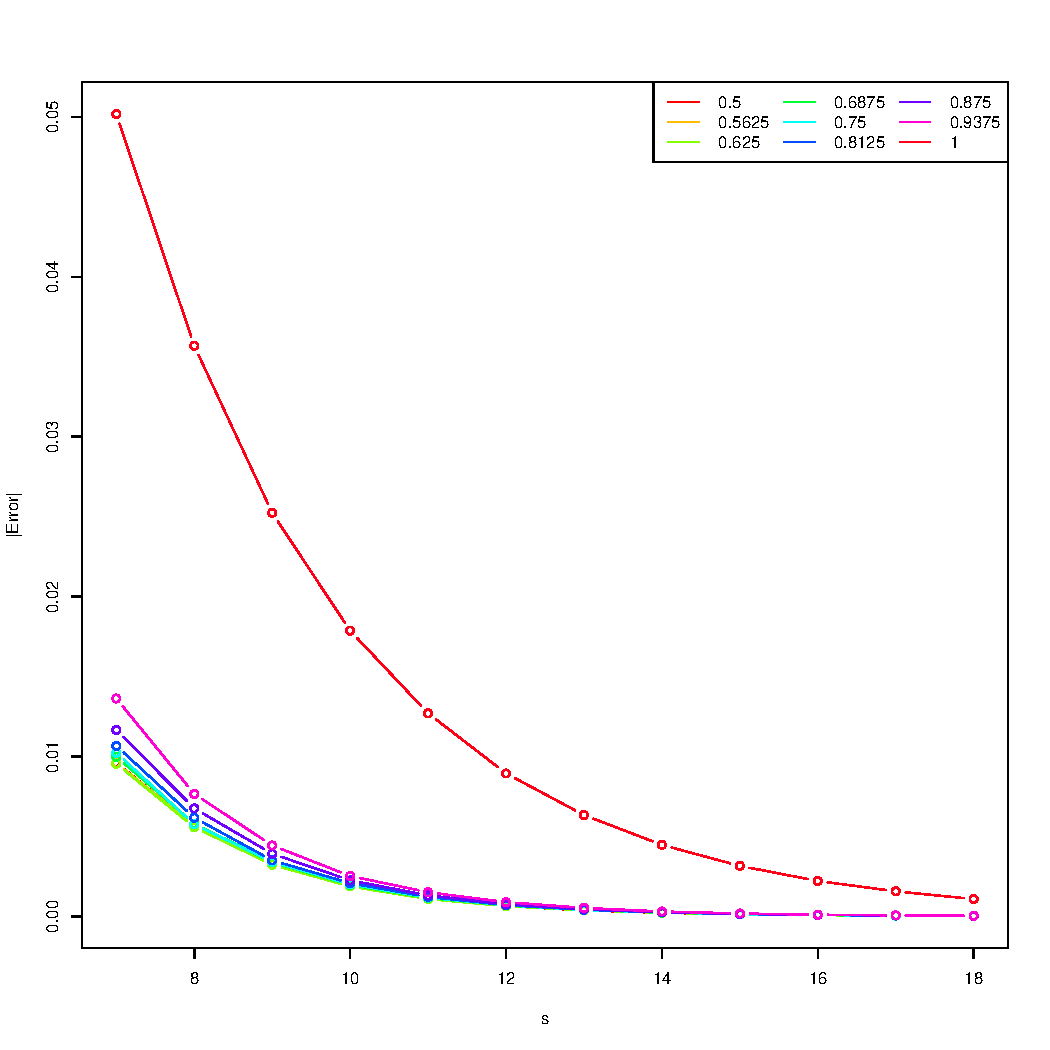
\includegraphics[scale=0.8]{nout_7_27a.pdf}
   \caption{Absolute error}
\end{figure}
 
 \begin{figure}[p]\label{f:lab}
   %\centering
   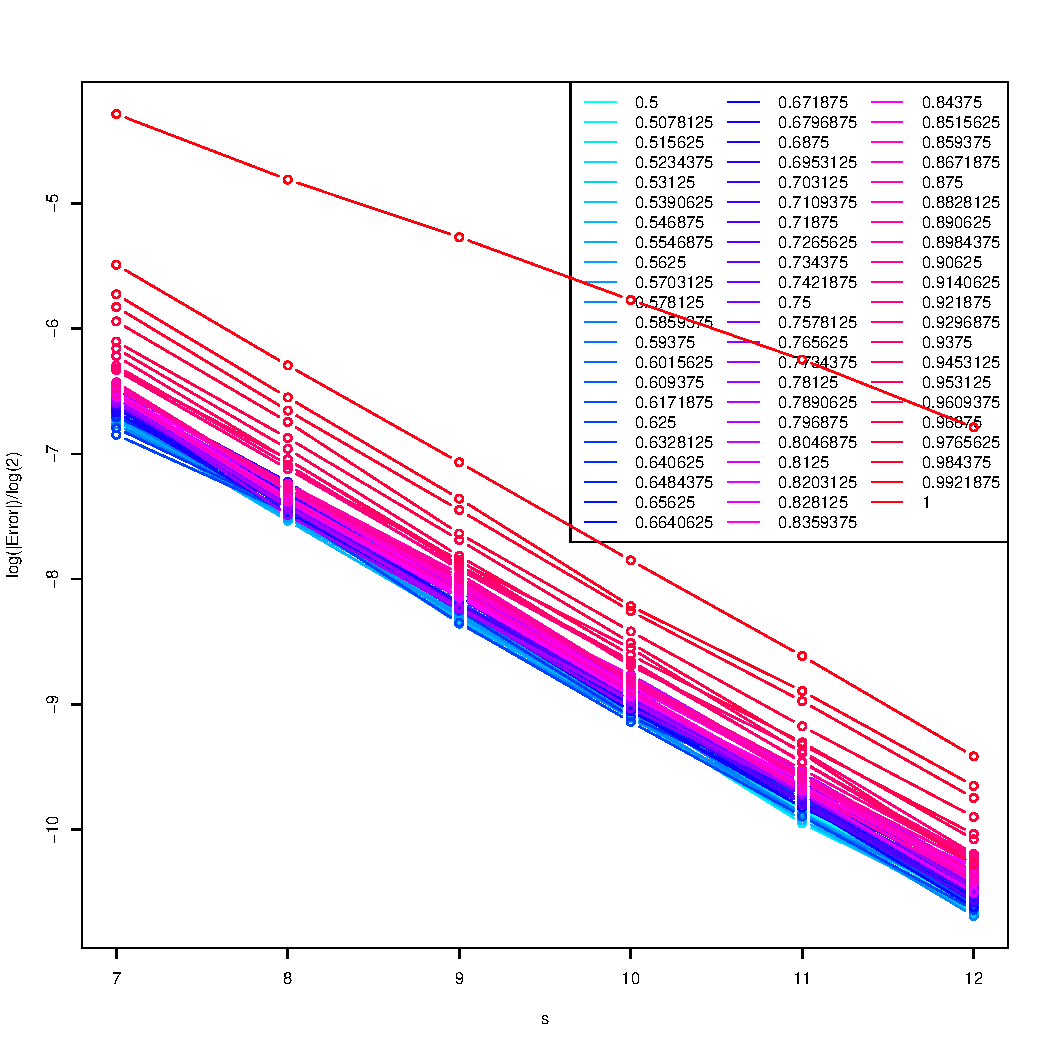
\includegraphics[scale=0.8]{nout_7_27alog.pdf}
   \caption{Logarithm of error} 
\end{figure}
 
 \begin{figure}[p]\label{f:ratio}
   %\centering
   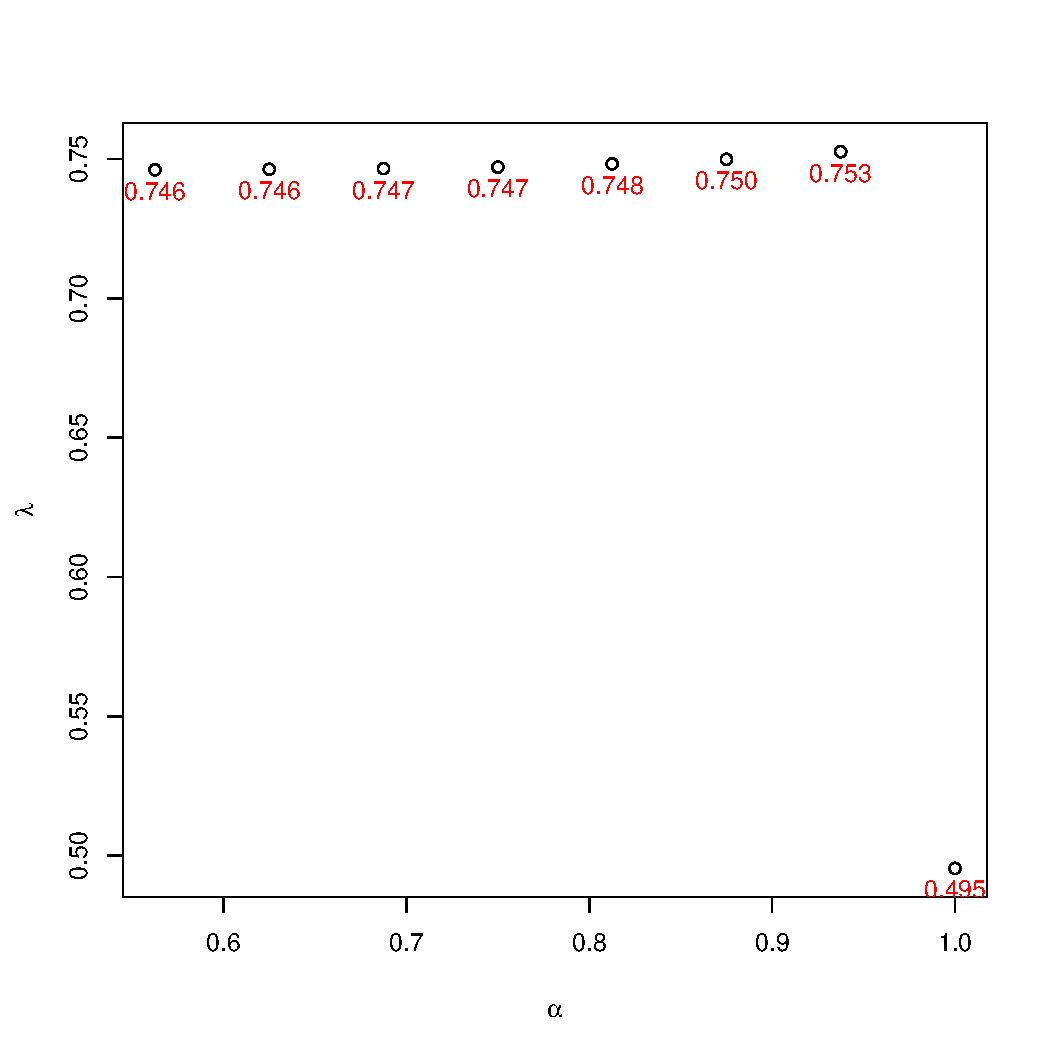
\includegraphics[scale=0.8]{nout_7_27arato.pdf} % requires the graphicx packagem 
   \caption{regression result of convergence rate}
\end{figure}

\subsection{An estimate of week discrete error}
\label{sec:de}

Let $S_k$ be a random walk (assume $S_0=0$)
with i.i.d increment, i.e.
$\Delta S_k = S_k -  S_{k-1}$ is i.i.d.
Define the ordered statistics $M_{k,n}$ be the $k$th smallest value in
$\Set{S_i}_{i=0}^n$.
Under this setting, clearly, $M_{0,n} = \inf_{0\leq i\leq n}S_i$
and $M_{n,n} = \sup_{0\leq i\leq n}S_i$
Define
\[S'_i = S_{i+k}-S_k\]
for fixed $k, n$.

In \cite{Wendel1960}, an identity about random walk with
i.i.d increment was derived:
\begin{equation}\label{eq:dpathdec}
(M_{k,n}, S_n) \eqlaw (\sup_{i\leq k} S_i +\inf_{i\leq n-k} S'_i, S_n)
\end{equation}

In \cite{Chaumont1999}, the author provides a combinatory treatment.
He constructed a explicit path transform for $S$ to $\tS$, such that
\[
(M_{k,n}, S_n) = (\sup_{i\leq k} \tS_i+\inf_{i\leq n-k} \tS'_i, \tS_n)
\]
Here $\tS$ has same distribution with $S$ and each path $S$
 one-one correspondence to $\tS$.

By using path transform, Chaumont proved
following continuous version of path decomposition:
\begin{equation}\label{eq:cpathdec}
(M_{\alpha,T}, S_T) \eqlaw (\sup_{t\leq \alpha{T}} S_T +\inf_{t \leq (1-\alpha)T} S'_t, S_T)
\end{equation}
where
\[
S'_t = S_{\alpha T+t} - S_{\alpha_T}.
\]

For Brownian motion case, this formula were proved in many different ways
and original due to \cite{Dassios1995}.


\cite{Janssen2008} give an estimate of the difference of  expectations
between maximum of Brownian motion and associated random walk.
Since we just give a really rough estimate, we only list the first two terms.
For $B_t$ a Brownian motion with drift $\mu$ and variance $1$ on time interval $[0,1]$, that is $B_t = \mu t + W_t$, where $W_t$ is standard Brownian motion, we can get
\begin{equation}\label{eq:est1}
E\max_{0\leq t \leq 1} B(t) - E\max_{n=0,\cdots, N}B(n/N)
= -\frac{\zeta(1/2)}{\sqrt{2\pi N}}-\frac{2g(1)-\mu}{4N} + O(1/N^{3/2})
\end{equation}
where
\[
g(t) = \mu \Phi(\mu \sqrt{t}) + \frac{1}{\sqrt{2\pi t}} e^{-\frac{1}{2}\mu^2 t}.
\]
\[
\zeta(1/2) \approx -3.92264613.
\]

For general Brownian $\tB(t)$ motion on time interval $[0,T]$ with drift $\tmu$, variance $\tsigma$,
we use following transform
\begin{align*}
\tB_t &= \tsigma \sqrt{T} B_{t/T} = \tsigma \sqrt{T} \mu t/T
+ \sqrt{T}\tsigma W_{t/T}\\
\mu &= \tmu \sqrt{T}/\tsigma
\end{align*}

\def\tg{\widetilde{g}}
We denote
\begin{equation}
\tg(\mu)=\mu \Phi(\mu) + \frac{1}{\sqrt{2\pi}} e^{-\frac{1}{2}\mu^2 }
\end{equation}

We derive the following formula:
\begin{equation}\label{eq:maxest}
\begin{split}
&E\max_{0\leq t\leq T} \tB(t) - E \max_{0\leq n \leq N} \tB(nT/N)\\ 
= & -\frac{\zeta(1/2)}{\sqrt{2\pi}}\tsigma \sqrt{T/N}
 -\frac{2\tg(\mu)-\tmu\sqrt{T} / \tsigma}{4N}\tsigma\sqrt{T} +
O(\sqrt{T}/N^{3/2})
\end{split}
\end{equation}

Now combine $(\ref{eq:cpathdec})$ $(\ref{eq:dpathdec})$ and $(\ref{eq:maxest})$, for $0 < \alpha < 1$,
we get an very rough estimate of the approximation order:
\allowdisplaybreaks
\begin{align*}
\E (M_{\alpha,T}) - \E (M_{k,N})
=& \EE{\sup_{t\leq \alpha{T}} S_t +\inf_{t \leq (1-\alpha)T}S'_t}
- \EE{\sup_{i\leq k} S_i+\inf_{i\leq N-k} S'_i}\\
=& \EE{\sup_{t\leq \alpha{T}} S_t +\inf_{t \leq (1-\alpha)T}S'_t
-  \sup_{i\leq k} S_i-\inf_{i\leq N-k} S'_i} \\
= &  \EE{\sup_{t\leq \alpha{T}} S_t - \sup_{i\leq k} S_i} +
\EE{\inf_{t \leq (1-\alpha)T} S'_t-\inf_{i\leq N-k} S'_i}\\
=& -\frac{\zeta(1/2)}{\sqrt{2\pi}}\tsigma \sqrt{\frac{\alpha T}{\alpha N}} - \frac{2\tg(\mu_1)-\mu_1}{4N}\tsigma\sqrt{\alpha T} +O(1/N^\frac{3}{2}) \\
&-\left(\frac{\zeta(1/2)}{\sqrt{2\pi}}\tsigma \sqrt{\frac{(1-\alpha)T}{(1-\alpha)N}} - \frac{2\tg(\mu_2) - \mu_2}{4N}\tsigma \sqrt{(1-\alpha)T} + O(1/N^\frac{3}{2})\right) \\
=& -\frac{\zeta(1/2) \tsigma}{\sqrt{2\pi}}\left(\sqrt{T/\alpha N}
\sqrt{\alpha} - \sqrt{T/(1-\alpha)N}\sqrt{1-\alpha}\right) \\
& - \frac{\tsigma\sqrt{T}}{4N}\left((2\tg(\mu_1)-\mu_1)\sqrt\alpha - (2\tg(\mu_2)-\mu_2)\sqrt{(1-\alpha)}\right) \\
&+ O(1/N^\frac{3}{2}) \\
=&- \frac{\tsigma\sqrt{T}}{4N}\left((2\tg(\mu_1)-\mu_1)\sqrt\alpha - (2\tg(\mu_2)-\mu_2)\sqrt{(1-\alpha)}\right) \\
& + O(1/N^{\frac{3}{2}}),
\end{align*}
where $k = \alpha N$, $\mu_1 =\tmu\sqrt{\alpha T}/\tsigma$, and $\mu_2 =\tmu\sqrt{(1-\alpha)T}/\tsigma$.
The third last equality holds by view $\inf_{t\leq (1-\alpha)T} S'_t$ as
$-\max_{t\leq (1-\alpha)T} (-S'_t)$.

This proof shows that the convergence order are all $1$ when $0<\alpha < 1$. When $\alpha = 0$ or $\alpha = 1$, the convergence rate is ${\frac{1}{2}}$. This partially explains the phenomenon that the strong convergence rate we discussed in section \ref{s:euler}.   %If $\alpha=1/2$ and the Brownian motion does not have  drift ($\mu=0$), it is easy to see (by noting that $\E M_{1/2,T} = \E -M_{1/2,T}$) $\E M_{1/2,T} = \E M_{k,N} = 0$.When the Brownian motion has drift, the order becomes $1$.

Using the same algorithm in section \ref{s:euler} Euler scheme and random walk,
we ran a simulation to examine the above claim. 
Here we first restate the parameter setting and algorithm.

The parameter setting is : 
\begin{equation}
\mu = 0 ; \sigma = 1; T=1; N = 2^b , 2^{b+1} , ... 2^{d} ; X_0 = 0; 
\alpha_j =  \frac{1}{2} + \frac{j}{2^b} , j = 0, 1 , 2..., 2^{b-1}
\end{equation}

The algorithm: 
\begin{enumerate}[1.]
\item Generate $2^{d}$ normal random sample $\Set{X_i}$ 
  with mean $\tmu=\mu/2^d$ ,
  $\tsigma = \sigma \sqrt {\frac{T}{2^b}}$  starting with $B_0 = 0$,
  add them up according to time and record them as
  $B_k = \sum_{1\leq i \leq k} X_i$.
\item Calculate the $\alpha_j$ quantiles 
  $M_{j,s}\triangleq M_{\alpha_j 2^s,2^s}$ for sequence 
  $\Set{B_k|k=i 2^{d-s}, 1\leq i\leq 2^{s}}$, where $b\leq s \leq d$. 
\item Use $M_{j,d}$ as the continuous quantiles $M(\alpha_j , T)$.
\item Repeat the above for $L$ times,
  get a sequence of data $\Set{M_{j,s}^{(l)}}_{1\leq l\leq L}$
\item Calculate the mean of errors for $s < d$:
\begin{align}
Err_{j,s} &= {\frac{1}{L}\left(\sum_{1\leq l \leq L} M_{j,d}^{(l)} - M_{j,s}^{(l)}\right)}
\end{align}
\end{enumerate}

We realize this algorithm for $d=27$,$b=6$ and generate more than 2000 sampled paths. As you can see in Figure \ref{f:err}, Figure \ref{f:lerr} and Figure \ref{f:rate}, the simulation results are coincident with our theoretical conclusion. 

\begin{figure}[p]\label{f:err}
   \centering
   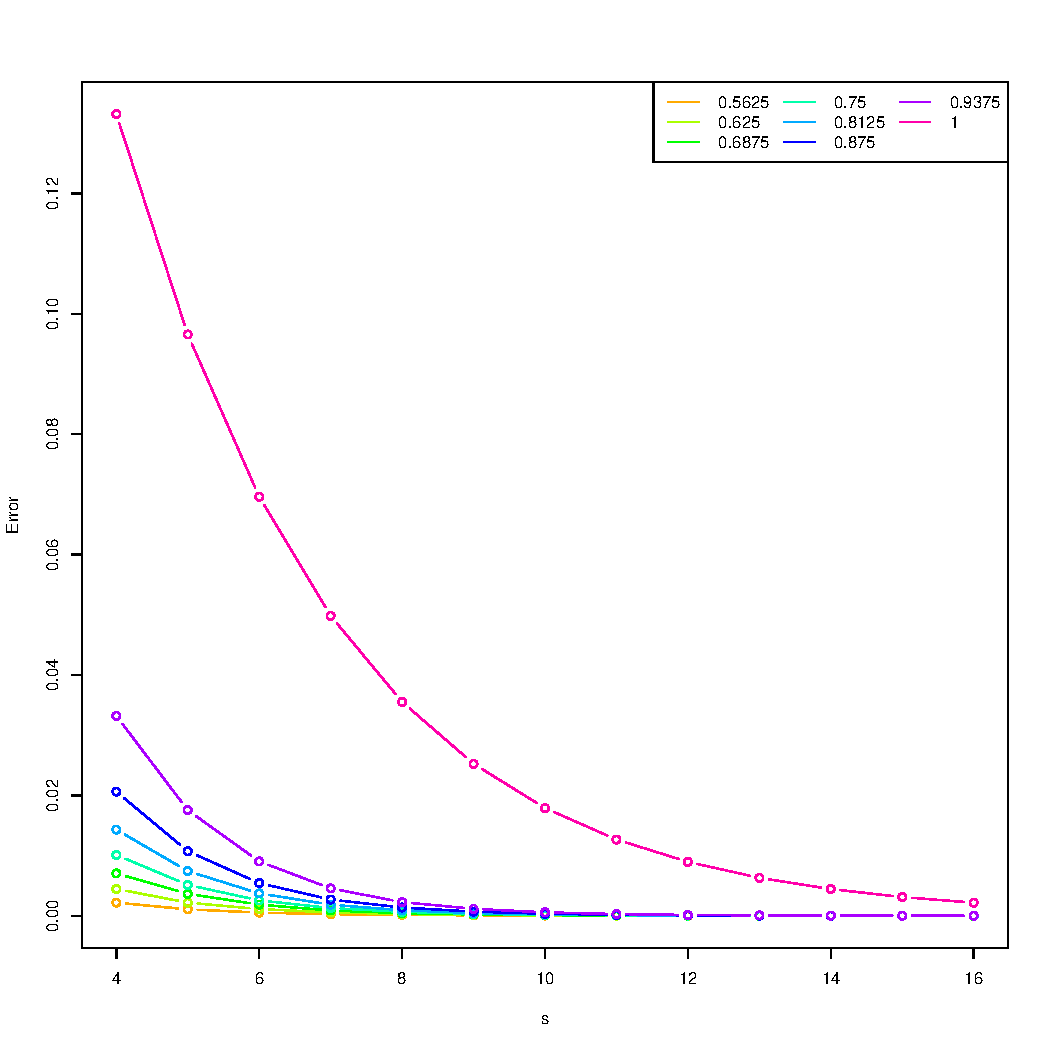
\includegraphics[scale=0.8]{nout_7_27.pdf} % requires the graphicx package
   \caption{ Errors }
\end{figure}

\begin{figure}[p]\label{f:lerr}
   \centering
   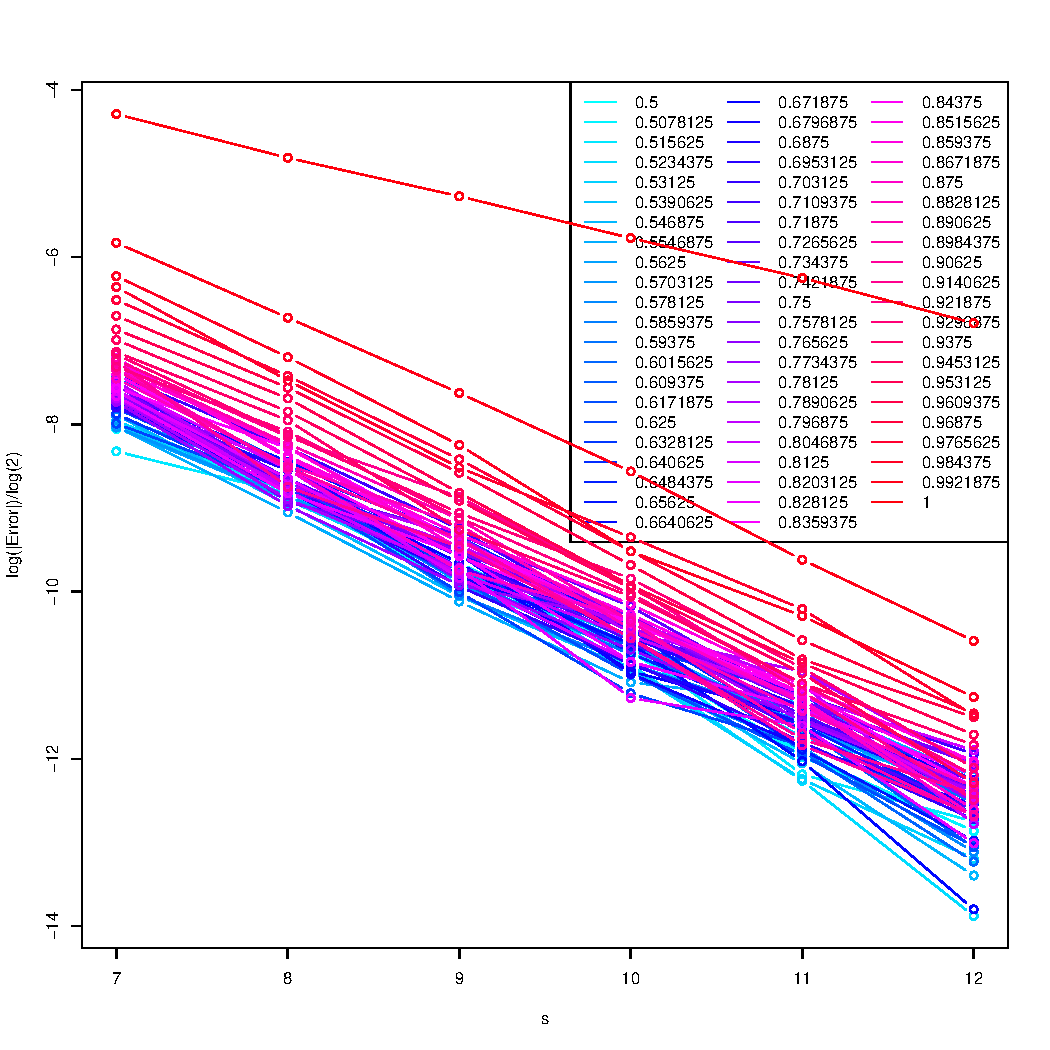
\includegraphics[scale=0.8]{nout_7_27log.pdf} % requires the graphicx package
   \caption{ Logarithm of Errors }
\end{figure}

\begin{figure}[p]\label{f:rate}
   \centering
   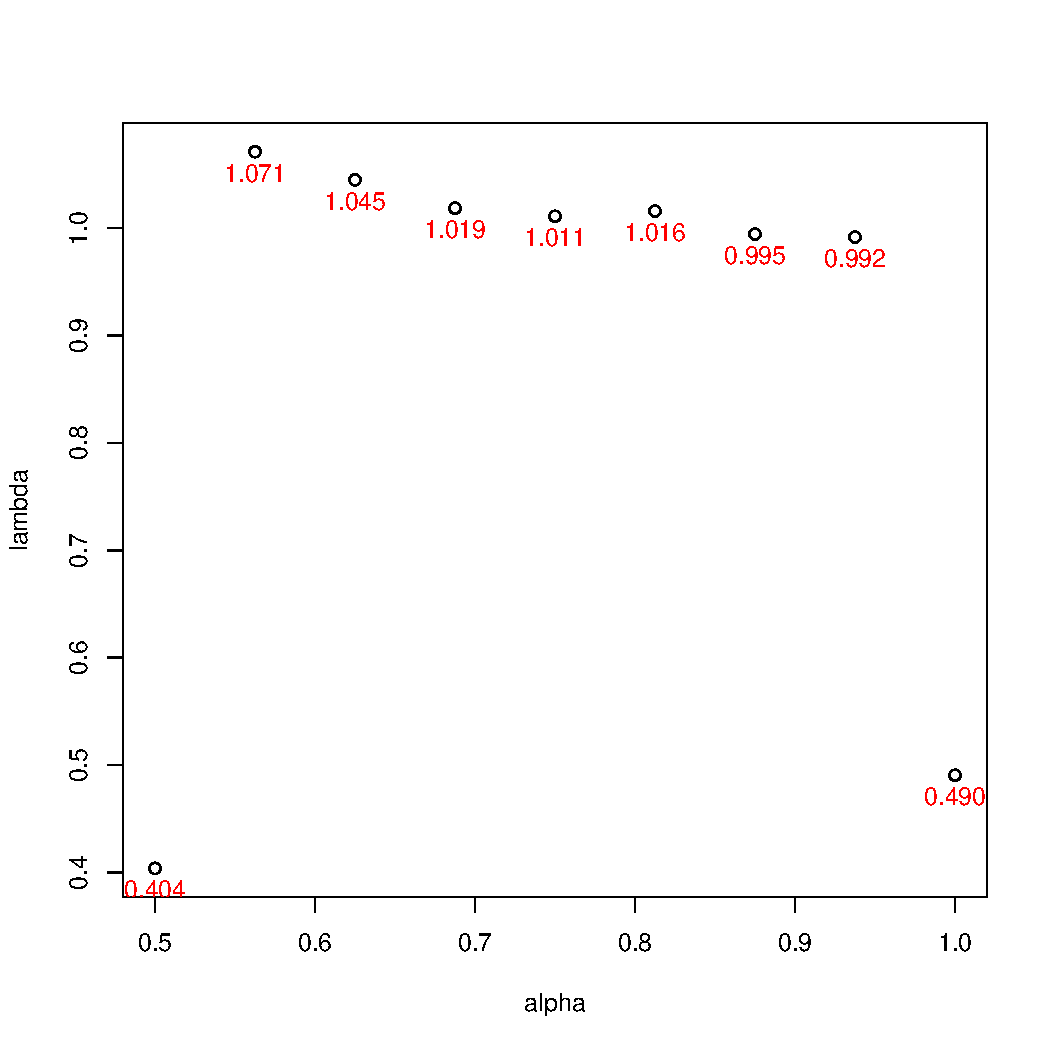
\includegraphics[scale=0.8]{nout_7_27rato.pdf} % requires the graphicx package
   \caption{ Convergence rate }
\end{figure}


Now, suppose that $f$ is an monotone Lipschitz continuous function.
Without loss of generality, ssume 
\begin{equation}\label{eq:lips}
0 \leq f(x)-f(y) \leq C (x-y) \quad \forall x>y,
\end{equation}
where some constant $C$. This always the case when $f$ the
(truncated) payoff of a $\alpha$-quantile option.

Then it is easy to see
\[
-C\left( \sup_{t\leq (1-\alpha)T} (-S'_i)-\sup_{i\leq n-k} (-S'_i)\right)
 \leq f(M_{\alpha,T}) - f(M_{k,N})
\leq  C \left(\sup_{t\leq \alpha{T}} S_t - \sup_{i\leq k} S_i\right)
\]
Hence
\begin{equation}\label{eq:liperr}
\abs{\E f(M_{\alpha,T}) - \E f(M_{k,N})}
\leq \max\Set{\sqrt{\alpha}, \sqrt{1-\alpha}}
C\frac{-\zeta(1/2)}{\sqrt{2\pi}}\sqrt{T/N}  + O(1/N)
\end{equation}

%By this, we can say the convergence rate of $\alpha$-quantile European option is at least 1/2.

\section{$\alpha$-quantile option}
\subsection{The advantage of $\alpha$-quantile option}
As we discussed before, lookback option is a path-dependent option with payoff calculated with the maximum or minimum price of the underlying asset during the life of the option. For example, a fixed strike lookback call option get the highest value obtained within the option's lifetime. In this case, to the holder, it can be viewed as a protection against large drop of stock price. This can be regarded as a method to deal with the unfavorable movement of a particular stock. The release of a prolonged lawsuit which may have a strong negative effect on the stock price. On the other side, lookback put option provides an insurance against large rises. But these characters also makes lookback options too expensive. Quantile option is one product that overcomes this shortcoming of lookbacks. Quantile option is cheaper than lookbacks, while it still provide partial protection against market movements. This property of quantile option was first discussed by \cite{Ballotta2001}.


Another advantage of quantile option is that the strong path dependence of its payoff make it immunize to possible market manipulation. Because the payoff of lookback using the maximum of stock price during option's lifetime. Particularly for at the money option close to maturity, which in this case are most vulnerable to the stock movement closing to maturity. Firms have influence on market price can use this advantage to leading market price move to their favorable direction. But since quantile option is strongly dependent, the manipulation effect is limited. 


\subsection{Tree method for European $\alpha$-quantile option}
\label{se:fsg}


Like lookback option, quantile option is also path-dependent. What makes things difficult is that quantile option is not markov. Normal tree methods which usually involve backward induction do not work in this case. We need to record all the information of the path because of lack of markov property, which will lead the tree to explosion computationally.
\cite{Kwok2001} proposed a special way to apply tree method to price quantile option. In this paper, they find a relation between the price of quantile option and the price of cumulative Parisian option. By this approximation, they can simplify the pricing of quantile option. In their paper, they assume that there are $M$ time steps for the whole monitoring period $[0,T]$, and they define ${S^M}_j$, $j = - M$, ...$0$,$1$,...,$M$ as the discrete asset prices at maturity. Under trinomial tree method, the possible prices happened in one tree are limited to $S^M_j$,  $j = - M$, ...$0$,$1$, ...,$M$, which is also true for the value taken by quantile of Brownian motion. Therefore they derived that
\begin{equation}\label{eq:kowk1}
V(\alpha, T) = e^{-rT} \sum^{M}_{j=-M}P[M(\alpha,T)=S^{M}_{j}]\max(S^{M}_{j}-X,0),
\end{equation}
where $V(\alpha,T)$ is for the value of $\alpha$-quantile option whose maturity it $T$, $P[M(\alpha,T)=S^{M}_{j}]$ is the probability that the quantile of Brownian motion achieve the value ${S^M}_j$,  $j = - M$, ...$0$,$1$, ...,$M$. In their paper, they observed that the difference between the prices of two cumulative Parisian binary options is a good approximation for $P[M(\alpha,T)=S^{M}_{j}]$ multiplies discount factor $e^{-rT}$, ie.
\begin{equation}\label{eq:kowk2}
e^{-rT}P[M(\alpha,T)=S^{M}_{j}] \approx V^{bin}_{cum}[(1-\alpha)T, S^{M}_{j-1}]-V_{cum}^{bin}[(1-\alpha)T, S_{j}^{M}]
\text{ for }j=-M, ... , 0, 1, ... , M
\end{equation}
where $V^{bin}_{cum}[d,B]$ is denoted as the price of continuously monitored cumulative Parisian binary option with down barrier $B$, and $d$ be the minimum cumulative time staying above the down barrier to avoid knock-out.


Combining equation (\ref{eq:kowk1})and (\ref{eq:kowk2}), they get
\begin{equation}\label{eq:kowk3}
V_{alp} = \sum^M_{j=-M} \max (S^M_j - X,0) \times \{V_{cum}^{bin}[(1-\alpha)T, S^M_{j-1}] - V^{bin}_{cum}[(1-\alpha)T, S^M_j]\} ,
\end{equation}
where $V^{bin}_{cum}[(1-\alpha)T, S_{-(M+1)}^M] = e^{-rT}$. By this result, we can turn pricing of quantile option into pricing of $2M+1$ cumulative Parisian option.


Parisian option is like an advanced version of barrier option. We know barrier options are options where the payoff depends on whether the underlying asset's price reaches a certain level (barrier) during the option's life. Barrier options usually trade in the over-the counter market. This kind of option is attractive because it is usually cheaper than similar option without barrier. Like vanilla option, barrier options also authorize holders the right to buy or sell, but  long sides of barrier options do not need to pay for scenarios they think is unlikely to happen in the future. One good example I find from Wikipedia is about IBM. If you believe that IBM will go up this year, but are willing to bet that it won't go above \$100, then you can buy the barrier and pay fewer premium than the vanilla option. But in this one-touch knock-out or knock-in can bring difficulties to option writers when asset price is close to barrier. Particularly in the foreign exchange market where manipulation of underlying asset price is not impossible. To overcome short period price manipulation, various adjustments to one-touch knock out or knock-in have been performed in practice. Parisian option is one solution.  In order to get activated, the underlying assets of Parisian option need to stay in the knout out or knout in region for certain period of time. The payoff of a cumulative Parisian option is dependent on the total amount of time the underlying asset price has spent above or below barrier. As for binary option, the payoff is either some fixed amount of some asset or nothing at all.



Kwok and Lau also proposed a forward shorting grid(FSG) to price cumulative Parisian option in \cite{Kwok2001}. The character of FSG is that this approach need add additional information at each node of  a lattice tree. Commonly in pricing path-dependent option, at each node we should add state vector to represent the path-dependent attribute, such as the extreme value of the underlying asset price achieved in lookback option case. As we know \cite{Hull1993} and \cite{Vijh1993} were the first authors suggested this approach. \cite{Barraquand1996} introduced a comprehensive framework for FSG. In this paper they indicated that the FSG method is unconditionally convergent. Further, they showed that when the covariance matrix is degenerate, the FSG method can outperform finite difference methods. The convergence of the FSG algorithm in pricing of Asian options was studied by \cite{Forsyth1999}.

In \cite{Kwok2001}, they constructed a trinomial tree to get the price of cumulative Parisian option. But due to the fact that the result is not steady according to the setting of the length of up movement between each immediate step, we modify their method to binomial tree.

In building binomial tree, we start by cutting the entire life of one option into many small time intervals of length $\Delta t = T / M$.
Our tree is build to mimic the logarithm process of underlying asset price. Denote $x=\ln S$. In each step, the logarithm of the price of underlying asset is assumed to move from its initial value of $x_0$ to one of the two new values, $x_0 + d + u$ and $x_0 + d - u$ with equal probability, that is $p_{up} = p_{down} = 0.5$ , where $u = \sigma \sqrt{\Delta t}$ and $d = (r - {\sigma}^2 /2)\Delta t$. Here $\sigma$, and $r$ are volatility and risk free interest rate, respectively. The model is illustrated in Figure~\ref{fig:tree1}.
\begin{figure}[p]
   \centering
   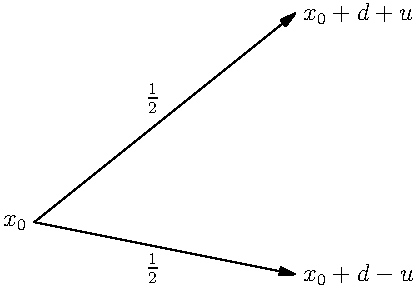
\includegraphics{trees.pdf} % requires the graphicx package
   \caption{Forward shooting}
   \label{fig:tree1}
\end{figure}

Like the notation used in \cite{Kwok2001}, we denote $V[m,j;k]$ as the numerical option value of the cumulative Parisian option at the $m$-th time interval,  $j$ upward jumps from the initial underlying asset value and $k$ times breaches so far. Let $g(k,j)$ be the grid function that describes the correlated evolution of number of breaches $k$ and price indicate $j$. Denote $x_j$ be the value of $x$ corresponding to $j$ upward movements on the binomial tree. Then we should add $1$ to the indicator $k$ if the underlying asset price $S$ is no more than the barrier $B$; i.e $x_j \leq \ln B$. Hence we can see that a suitable setting of the grid evolution function $g(k,j)$ should be
\begin{equation}\label{eq:grid}
g(k,j) = k + 1_{\Set{x_j \leq B}}
\end{equation}
where $1_{\set{x_j \leq B}}$ is the indicator function. It is defined as
\begin{equation}\label{eq:grid-indicator}
1_{\Set{x_j \leq B}} =  \begin{cases}
1 & \text{if } x_j \leq \ln B \\
0 & \text{if } x_j > \ln B
\end{cases}
\end{equation}
Then the FSG method for pricing the cumulative Parisian binary option can be expressed as
\begin{equation}\label{eq:fsg}
V[m-1,j;k] =\set{0.5V[m,j+1;g(k,j+1)]+0.5V[m,j-1,g(k,j-1)]}e^{-r\Delta t}
\end{equation}
for $m-1 < M$.


Let $N$ be the predetermined number of breaches recoreded for the all duration of the life of an option that is desired to activate   the contract.
Considering the binary feature of the option, we should initiate our algorithm with
\begin{equation}\label{eq:initiate}
V[M,j;k] = \begin {cases}
1 & \text{if }  k < N \\
0 & \text{if }  k \geq N
\end{cases}
\end{equation}
By (\ref{eq:initiate})  (\ref{eq:fsg}) and backward induction, we can get the price of cumulative Parisian binary option with any prescribed times of breaches and barrier.

Recall what we get by equation (\ref{eq:kowk2}). In order to get the price of $\alpha$-quantile option, we can use the prices of $2M + 1$ cumulative Parisian binary options to approximate $\alpha$-quantile option's value. Hence using the FSG method we described above to calculate the prices of cumulative Parisian option  and doing a simple math work by equation (\ref{eq:kowk2}), we can get the approximated price for $\alpha$-quantile option with $M$ time steps.

Recall we defined earlier $\Delta t = T / M$. We compute the approximated option price of an $\alpha$-quantile call option with different time steps using equation (\ref{eq:kowk2}). As you can see in Figure (\ref{fig:2}),
the numerical values of option are plotted against varying $\Delta t$. The values of parameters of the $\alpha$-quantile call option are set as: $\alpha = 0.8$, $S_0 = 100$, $X = 95$, $r = 5\%$, $\sigma = 20\%$, and $T = 0.25$.
\begin{figure}[htbp]
   \centering
   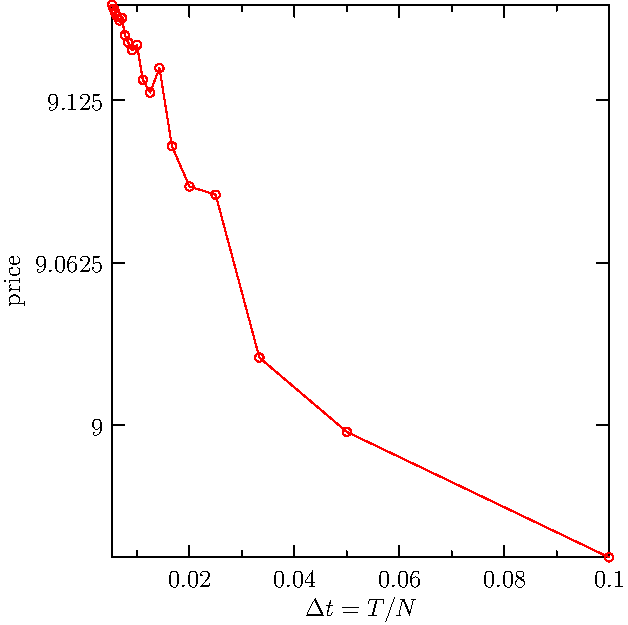
\includegraphics{bfsg.pdf} % requires the graphicx package
   \caption{FSG result}
   \label{fig:2}
\end{figure}




%\subsection{A static hedging for $\alpha$-quantile put option}
Inspired by the approximation of quantile option using cumulative Parisian options, we here propose a static hedging of quantile options using cumulative binary Parisian options. As we discussed earlier, the payoff of a cumulative binary Parisian option is that: only if the price of stock spend enough time under a predetermined barrier, its payoff is \$1; otherwise, its payoff is 0, it is worth nothing. We explicitly account for the discreteness of the tick size. That is the value of stock price only can be multiples of 1/8. Then for a put quantile option, the intuition for our hedging lies in the ability to rephrase the question, what was the certain quantile of stock price as several questions. 

For example, for $40\%$-quantile put option with stock price started from 1 and strike price 2, we can replicate its payoff using cumulative Parisian options which are alive only if they spend more than $0.4*T$ time under their barrier. For the quantile option, it has payoff only if the $40$ percentile is less than 2, the strike price. Also it is obvious that $40$ percentile must be larger than 0. In this sense, we hold 0.125 share of each cumulative binary Parisian binary option with barrier raging from $0.125. 0.250, 0.375.�, 2$.  If in the end of maturity, the 40 percentile of stock price is larger than 2, the quantile option gets nothing. Since the 40 percentile is larger than 2, then the stock price must be under 2 for less than 40$\%$ of the time before maturity. In this case all the binary option gets nothing. But if the quantile is $1.750$, the quantile option gets a payoff of $0.250=2-1.750$. While for the binary options, in this case, options with barrier $2$ and $1.875$ are alive. The payoff you can get from binary options is $0.125*2=0.250$. That is the payoff of the collections of binary options is identical to your quantile option. These are true for other scenarios of the value of quantile.  In other words, by holding a collection of cumulative Parisian binary option, we can realize a static hedging.

Probably, you have already found out that this scheme only works for European puts, because that you can find the two side boundary of effective quantile. This condition is not true for calls. 


\subsection{A tree method for American $\alpha$-quantile option}
Non-markov property of  the quantile of Brownian motion cause serious problem 
when we want to use tree method. We need to record all the information alone the
path, at least, we have to record the occupation time of $X_k$.
 
In risk neutral world, we always can write the price of 
American option in following way:
\[
C = \sup_{\tau\leq T} Ef(X_\tau^\alpha,\tau),
\]
where $\tau$ are any stopping time stops before $T$, 
\[
f(x,t) = 
\begin{cases}
e^{-rt}(x-K)^+ & \text{for call option}\\
e^{-rt}(K-x)^+ & \text{for put option}
\end{cases}
\]
as usual.
This is an optimal stopping problem. 

The obvious way to solve this numerically, is using tree method. 
Discrete the time, i.e. let $0=t_0< t_1, \cdots, t_n$.
Let $P_k=(X_0, \cdots, X_k)$ be a path of Geometric Brownian motion, 
Then $X_{k+1}$ can only be $X_{k}+u$ and $X_{k}-d$ in probability
$p^+$ and $p^-$  where $u,d,p^+$ and $p^-$ are prefixed 
constants in usual binomial tree method, each will .
Then let 
\[
\mathrm{Pay}_{P_j} = e^{rt_j}f(X_{P_j}^\alpha, t_j)
%=
%\begin{cases}
%(x-K)^+ & \text{for call option}\\
%(K-x)^+ & \text{for put option}
%\end{cases}
\] 
be the payoff if the option holder execute the option at time $t_j$, 
where $X_{P_n}^\alpha$ denotes the $\alpha$-quantile of path $P_n$. 
For $n$, let 
\[
C_{P_n} = \mathrm{Pay}_{P_n}
\]
For $j< n$, 
let 
\[
C_{P_j} = \max\Set{E_{P_j}, \mathrm{Pay}_{P_j}}
\]
where
\[
E_{P_j} = e^{-r(t_{j+1}-t_j)}(p^+C_{(P_j,X_j+u)} + p^-C_{(P_j,X_j-d)})
\]
is the expectation return if the holder of the option
do not execute his right at time $t_j$, providing the historical data of 
the stock price is given by $P_j$. 

Now the optimal stopping time is given by 
\[
\tau(P_n) = \inf\Set{t_j| Pay_{P_j}\geq E_{P_j}}
\]
here $P_j$ is the restriction of $P_n$ at $(t_0, \cdots, t_j)$, i.e. 
\[
P_j = (X_0, \cdots, X_j) \text{ if } P_n=(X_0, \cdots, X_n). 
\] 

Hence $C_{(0)}$ is the price of American $\alpha$-quantile option at time $t_0$. Based on this observation, we have a recurrence relation for computing $C_{(0)}$.

It is nature to realize this scheme by using the ``Depth First Search'' algorithm. Depth first search (DFS) is an standard algorithm for visiting all nodes and generating all possible path in a tree. The character of this method is that we start form the root of a tree and explore as deep as possible until the end of each branch before backtracking. In practice, we build the tree with depth $n+1$, each non-leaves nod has two children corresponding to $\Set{X_j+u,X_j-d}$. Hence the complexity of this ``brute force'' method is $O(2^n)$. It is clear that all the nodes at depth $j$ correspond to one and only one path $P_j$. So we label the node by $N_{P_j}$.  For any node, say $N_{P_j}$, we first compute $C_{P_{j+1}}$, where the possible $N_{P_{j+1}}$ are all of its two children. After visiting all its children and computing $C_{P_{j+1}}$, it backtracks to node $N_{P_j}$, and computes $E_{P_j}, Pay_{P_j}$ and then $C_{P_j}$. After that, it goes back to the parent of $N_{P_j}$. Now we apply the same process to $N_{P_{j-1}}$  as we do to $N_{P_{j}}$. In other words, if it does not finish visiting all its children, it will visit the next one; if it finishes visiting all the children, it will compute the value of the note and go back to its parent. 

Because the computational time of this method is going exponentially as the steps increasing. It is very time consuming to obtain an result with large steps. To solve this question, we propose an extrapolation method to improve the converge speed.

Richardson extrapolation is a method to accelerate the sequence convergence rate first studied by \cite{Richardson}.
Let $v(h)$ be the approximate price of the option got from the tree method with step length $h$. Suppose the tree method is of order $\gamma$.  
We have 
\[
v(h) = v_0 + Ch^\gamma + o(h^\gamma)
\]
where $v_0$ is the true value of the $\alpha$-quantile option.
Now we compute for two different step length $h_1, h_2$. 
Then 
\begin{align}
h_1^\gamma v(h_2) &= v_0 h_1^\gamma + C(h_1h_2)^\gamma + o(h_2^\gamma) \label{eq:exs1}\\
h_2^\gamma v(h_1) &= v_0 h_2^\gamma + C(h_1h_2)^\gamma + o(h_1^\gamma) \label{eq:exs2}
\end{align}
Consider (\ref{eq:exs1})-(\ref{eq:exs2}),
we get
\[
v_0(h_1^\gamma - h_2^\gamma) \approx h_1^\gamma v(h_2) - h_2^\gamma v(h_1)
\]
i.e. 
\[
v_0 \approx \frac{ h_1^\gamma v(h_2) - h_2^\gamma v(h_1)}{
  h_1^\gamma - h_2^\gamma}
= \frac{\eta^\gamma v(h_2) - v(h_1)}{\eta^\gamma -1 },
\]
where $\eta = h_1/h_2$.

In our case, denote $C_n$ be the value corresponding to $n$ steps. Based on the conclusion in section \ref{sec:de}, it is reasonable to assume that our tree method converges on order 1. That is $\gamma = 1$. 
Then the true value of $\alpha$-quantile option 
\[
C_\infty \approx \frac{\eta C_{n_2} - C_{n_1}}{\eta-1},
\]
where $\eta = (T/n_1)/(T/n_2) = n_2/n_1$.
This is the general form of Richardson extrapolation.
If take $n_2=2n, n_1=n$, we get the usual Richardson extrapolation formula
\[
C_\infty \approx 2 C_{2n} - C_n. 
\]

Because there is no other method to price American $\alpha$-quantile option so far. In other words, there does not exist direct result acting as an comparing standard. However, since conceptually our tree should also work for European $\alpha$-quantile option, here we first compare the results using this tree method with value obtained by other method.


The results with parameters 
\[
K=100, r=0.05, \sigma=0.2, \alpha=0.5, T=1
\]
can be seen in Table~\ref{fig:euro5}


\begin{table}[p]
\caption{European $\alpha$-quantile option, with parameter
	$K=100, r=5\%, \sigma=0.2, \alpha=0.5, T=1$. 
	The extrapolation is based on results got at 28 steps and 36 steps. Data in last line is from \cite{Laura2001}.}
\begin{center}
\begin{tabular}{l|lllllll}
 $S_0$ & $90$ & $95$ & $100$ & $105$ \\
\hline
28 steps & 1.60216 & 3.17876 & 5.61323 & 8.92661\\
30 steps & 1.60443 & 3.17806 & 5.61404 & 8.92702\\
32 steps & 1.60637 & 3.18346 & 5.61678 & 8.92718\\ 
34 steps & 1.60435 & 3.18426 & 5.61758 & 8.92875\\
36 steps & 1.60411 & 3.18846 & 5.61940 & 8.92925\\
\hline
Extrapolation & 1.61094 & 3.22241 & 5.64100 & 8.938490 \\
\hline
Paper & 1.6588 & 3.2695 & 5.7501 & 9.0895\\
\hline
lookback & 9.45696 & 13.86499 & 19.16763 & 24.88215
\end{tabular}
\end{center}
\label{fig:euro5}
\end{table}%

In Table~\ref{fig:euro8}, for parameter setting as $\alpha = 0.8$, $K = 95$, $r = 5\%$, $\sigma = 20\%$, and $T = 0.25$, we present the results got by our tree method and Forward Shooting Grid discussed in section \ref{se:fsg}.


\begin{table}[p]
\caption{European $\alpha$-quantile option, with parameter
	$K=95, r=5\%, \sigma=0.2, \alpha=0.8, T=0.25$. 
	The extrapolation is based on results got at 28 steps and 36 steps.}
\begin{center}
\begin{tabular}{l|lllllll}
$S_0$ & $95$ & $100$ & $105$        \\
\hline
26 & 4.59876 & 9.10824 & 14.1838  \\
28 & 4.60931 & 9.11777 & 14.1954 \\
30 & 4.61547 & 9.12485 & 14.2030 \\
32 & 4.61816 & 9.12648 & 14.2054  \\
34 & 4.61785 & 9.12676 & 14.2051 \\
36 & 4.62050 & 9.12908 & 14.2079 \\
extrapolation & 4.659665 & 9.168665 & 14.25165\\
FSG & 4.66082 & 9.16298 & 14.2309 \\
lookback & 8.381566 &  13.76059 & 19.13961
\end{tabular}
\end{center}
\label{fig:euro8}
\end{table}%

Comparing the results by our tree method with extrapolation, Forward shooting grid and Monte Carlo method, we think our tree method is correct and efficient. Since, as we checked, it works well for European $\alpha$-quantile option, it should also work for American style $\alpha$ quantile option. 

For parameters setting as
\[
K=100, r=0.05, \sigma=0.2, \alpha=0.5, T=1
\]
, with our tree method, we get the price of American $\alpha$-quantile option in Table \ref{fig:amer5}. Comparing data in Table \ref{fig:euro5} and Table \ref{fig:amer5}, we can see price for American option is more expensive than European option with same feature. This again insures that our method is correct. 
 
\begin{table}[p]
\caption{American $\alpha$-quantile option, with parameter
	$K=100, r=0.05, \sigma=0.2, \alpha=0.5, T=1$. 
	The extrapolation is based on results got at 28 steps and 36 steps.}
\begin{center}
\begin{tabular}{l|lllllll}
$S_0$ & $90$ & $95$ & $100$ & $105$ \\
\hline
26steps & 1.69411 & 3.43582 & 6.19546 & 10.2276 \\
28steps & 1.70066 & 3.44695 & 6.21365 & 10.2465 \\
30steps & 1.70434 & 3.45157 & 6.22887 & 10.2624 \\
32steps & 1.70651 & 3.45927 & 6.24320 & 10.2738  \\
34steps & 1.70590 & 3.46373 & 6.25529 & 10.2831 \\
36steps & 1.70711 & 3.47019 & 6.26644 & 10.2891 \\
Extrapolation & 1.729685 & 3.551530 & 6.451205 & 10.43820 \\
\end{tabular}
\end{center}
\label{fig:amer5}
\end{table}%

\begin{table}[p]
\caption{American $\alpha$-quantile option, with parameter
	$K=95, r=5\%, \sigma=0.2, \alpha=0.8, T=0.25$. 
	The extrapolation is based on results got at 28 steps and 36 steps.}
\begin{center}
\begin{tabular}{l|lllllll}
$S_0$ & $95$ & $100$ & $105$        \\
\hline
26 & 4.84702 &  9.68628 & 14.8771 \\
28 & 4.85892 &  9.70169 & 14.8932\\
30 & 4.86696 &  9.71225 & 14.9049\\
32 & 4.87621 &  9.72318 & 14.9164\\
34 & 4.88228 &  9.73134 & 14.9251\\
36 & 4.88821 &  9.73857 & 14.9329\\
extrapolation & 4.990725 & 9.867650&  15.07185
\end{tabular}
\end{center}
\label{fig:amer8}
\end{table}%




\section{Connect the discrete and continuous $\alpha$-quantile options}
We follow \cite{Broadie1999}.

In this section we omit the subscript $\alpha$ and $k$. Denote 
$M$ and $M_m$ be the $\alpha$ quantile of Brownian motion with drift $\mu$ 
and variance $\sigma$ at time $T$ and its step length $T/m$ version
 respectively. 

From the previous section, we know the mean of discrete error satisfies
\[
E(M-M_m) = \beta /m + O(m^{-\frac{3}{2}}),
\]
where 
\[
\beta = - \frac{\tsigma\sqrt{T}}{4}\left((2g'(\mu_1)-\mu_1)\sqrt{\alpha} 
  -(2g'(\mu_2)-\mu_2)\sqrt{(1-\alpha)}\right).
\]

We find 
\[
\begin{split}
 & E(e^{M_m} - x)^+ \\
=& 
E(e^M-x)^+ - E(e^M-e^{M_m}; e^M,e^{M_m}>x)\\
&+E(e^{M_m}-x;e^{M_m}\geq x > e^M)
-E(e^M-x;e^M\geq x > e^{M_m})\\
=& A - B + C + D
\end{split}
\]

Assume $m(e^M-e^{M_m})$ convergence in distribution to some random variable $U$.
Then, 
\[
0 \leq C \leq E(e^{M_m}-e^M;e^{M_m}\geq x > e^M)
\] 
Since $P(e^{M_m}\geq x > e^M) \rightarrow 0$,
\[
E(m(e^{M_m}-e^M);e^{M_m}\geq x > e^M) \rightarrow 0
\]
by the uniformly integrability. So $C$ and similarly $D$ is $o(1/m)$.
If the assumption is not true, if we can prove
\begin{equation}
E(e^{M_m}-e^M;e^{M_m}\geq x > e^M) \sim o(1/m) \label{eq:sp1}
\end{equation}
it is also OK. 

Now, 
\begin{align}
  B =&  E(e^M-e^{M_m}; e^M,e^{M_m}>x) \notag \\
  =& E(e^M-e^{M_m}; e^M>x) -  E(e^M-e^{M_m}; e^{M_m}<x<e^M) \notag \\
  =& E(e^M-e^{M_m}; e^M>x) + o(1/m) \notag \\
  =& E(e^M \beta/m;e^M>x) +o(1/m) \label{eq:sp2}
\end{align}

Hence,
\begin{align}
 & E((e^{M_m}-x)^+) \notag\\
=& E((e^M-x);e^M>x) - E(e^M \beta/m;e^M>x) + o(1/m) \notag\\
=& E(e^M(1-\beta/m)-x;e^M>x) + o(1/m) \notag \\
=& E[e^{M-\beta/m}-x;e^M>x] + o(1/m) \label{eq:cor1}\\
=& e^{-\beta/m}E(e^M-xe^{\beta/m};e^M>x) + o(1/m) \notag\\
=& e^{-\beta/m}E(e^M-xe^{\beta/m};e^M>xe^{\beta/m})  \notag\\
 & +e^{-\beta/m}E(e^M-xe^{\beta/m};e^M\in [xe^{\beta/m}, x])  + o(1/m)\label{eq:sp3}\\
= & e^{-\beta/m}E[e^M-xe^{\beta/m};e^M>xe^{\beta/m}] + o(1/m) \\
= & e^{-\beta/m}E[(e^M-xe^{\beta/m})^+] + o(1/m) \label{eq:cor2}
\end{align}
Now both equation (\ref{eq:cor1}) and (\ref{eq:cor2}) 
are correction formulas.


For equation (\ref{eq:sp3}),
\[
\begin{split}
&|E(e^M-xe^{-\beta/m};e^M\in [xe^{-\beta/m}, x])|\\
\leq& x|1-e^{-\beta/m}|P(M \in [\log x,\log x -\beta/m])\\
=& O(1/m)O(1/m) = o(1/m) 
\end{split}
\]
The inequality is obtained by observation. The second is because the density function is finite and Cauchy-Schwarz inequality.

\def\bM{\overline{M}}
\def\darrow{\xrightarrow{\mathcal{D}}}
\def\Cov{\mathrm{Cov}}
Now we discuss the equation (\ref{eq:sp2}).
Use Taylor expansion, we get
\[
e^{M_m}-e^M = e^M(M_m-M) + \frac{1}{2}e^{\bM_m}(M_m-M)^2
\]
for some $\bM_m$ between $M$ and $M_m$.

Similarly, to get equation (\ref{eq:cor1}), using Taylor expansion, we find
\[
e^{M-\frac{\beta}{m}}= e^{M} - e^M(M-\frac{\beta}{m}-M) + \frac{1}{2}e^{\tM_m}(M-\frac{\beta}{m}-M)^2
\]
for some $\tM_m$ between $M-\frac{\beta}{m}$ and $M$. 


Now assume 
\[
m^\gamma(M-M_m)=W_m \darrow W,
\]
where $\gamma > \frac{1}{2}$ as we see in the simulation.
As later, we will prove $e^{\bM_m}m^{2\gamma}(M-M_m)^2$ is uniformly integrable.
So 
\[
m^{2\gamma}(E[e^M]-E[e^{M_m}] - E[e^M(M-M_m)])\darrow C,
\]
for some constant. 
Hence, 
\begin{align}
&E[e^M]-E[e^{M_m}] \notag \\
=& E[e^M(M-M_m)] + C m^{-2\gamma} +o(m^{-2\gamma}) \notag\\
=& E[e^M]E[M-M_m] + \Cov(e^M,M-M_m) + o(1/m) \notag\\
=& E[e^M]\beta/m +  \Cov(e^M,M-M_m) + o(1/m)\notag\\
=& E[e^M]\beta/m + o(1/m) \label{eq:sp4}
\end{align}
To varify equation (\ref{eq:sp4}) we need to justify 
\[
\Cov(e^M,M-M_m)\sim o(1/m),
\]
by uniformly integrability argument? 

To check the uniformly integrability of $e^{\bM_m}m^{2\gamma}(M-M_m)^2$,
we use the Schwarz ineuality.
\[
E[(e^{\bM_m}m^{2\gamma}(M-M_m)^2)^2]
\leq E[e^{4\bM_m}] E[(m^{2\gamma}(M-M_m))^4]
\]
But, we have 
\[
\sup_mE[e^{p\bM_m}] \leq E[e^p\max_{0\leq t\leq T}B_t] < \infty \quad \forall p>0.
\]
If we have 
\[
\sup_m E[|m^{2\gamma}(M-M_m)|^4] \leq \infty
\]
we can prove the uinformly integrability. 

In fact, we can modify this proof by using H\"older's inequality, then 
we only need
\[
\sup_m E[|m^{2\gamma}(M-M_m)|^p] < \infty 
\]
for some $p>2$. 



\bibliography{prob}

\end{document}  